% !TEX encoding = UTF-8 Unicode

% Compilation using 'acmsmall.cls' - version 1.3 (March 2012), Aptara Inc.
% (c) 2010 Association for Computing Machinery (ACM)
%
% Questions/Suggestions/Feedback should be addressed to => "acmtexsupport@aptaracorp.com".
% Users can also go through the FAQs available on the journal's submission webpage.
%
% Steps to compile: latex, bibtex, latex, latex


\documentclass[prodmode,acmtochi]{acmsmall} % Aptara syntax

% Package to generate and customize Algorithm as per ACM style
\usepackage[ruled]{algorithm2e}
\renewcommand{\algorithmcfname}{ALGORITHM}
\SetAlFnt{\small}
\SetAlCapFnt{\small}
\SetAlCapNameFnt{\small}
\SetAlCapHSkip{0pt}
\IncMargin{-\parindent}

% Packages
\usepackage[super]{nth}
\usepackage[inline]{enumitem}
\usepackage{moreenum}
\usepackage{tabu}
\usepackage{booktabs}
\usepackage{array}
\newcommand{\ra}[1]{\renewcommand{\arraystretch}{#1}}
\newcommand{\urlhttp}[1]{\href{http://#1}{\nolinkurl{#1}}}
\newcommand{\urlhttps}[1]{\href{https://#1}{\nolinkurl{#1}}}

% Metadata Information
\acmVolume{9}
\acmNumber{4}
\acmArticle{39}
\acmYear{2010}
\acmMonth{3}

% Copyright
%\setcopyright{acmcopyright}
%\setcopyright{acmlicensed}
%\setcopyright{rightsretained}
%\setcopyright{usgov}
%\setcopyright{usgovmixed}
%\setcopyright{cagov}
%\setcopyright{cagovmixed}

% DOI
\doi{0000001.0000001}

%ISSN
\issn{1234-56789}

% Document starts
\begin{document}

% Page heads
\markboth{B. Harmon et al.}{Embodied Spatial Cognition in Tangible Computing}

% Title portion
\title{Embodied Spatial Cognition in Tangible Computing} % Spatial Performance in Tangible Computing 
\author{BRENDAN ALEXANDER HARMON
\affil{North Carolina State University}
ANNA PETRASOVA
\affil{North Carolina State University}
VACLAV PETRAS
\affil{North Carolina State University}
HELENA MITASOVA
\affil{North Carolina State University}
ROSS ​KENDALL MEENTEMEYER
\affil{North Carolina State University}
EUGENE BRESSLER
\affil{North Carolina State University}
ART RICE
\affil{North Carolina State University}}

\begin{abstract}
%
\end{abstract}

%
% The code below should be generated by the tool at
% http://dl.acm.org/ccs.cfm
% Please copy and paste the code instead of the example below. 
%
\begin{CCSXML}
<ccs2012>
<concept>
<concept_id>10003120.10003121</concept_id>
<concept_desc>Human-centered computing~Human computer interaction (HCI)</concept_desc>
<concept_significance>500</concept_significance>
</concept>
<concept>
<concept_id>10003120.10003121.10003122.10011749</concept_id>
<concept_desc>Human-centered computing~Laboratory experiments</concept_desc>
<concept_significance>500</concept_significance>
</concept>
</ccs2012>
\end{CCSXML}

\ccsdesc[500]{Human-centered computing~Human computer interaction (HCI)}
\ccsdesc[500]{Human-centered computing~Laboratory experiments}
%
% End generated code
%

\keywords{Human-computer interaction, tangible interfaces, interaction design, physical computation, embodied cognition, spatial thinking, geospatial modeling}

\acmformat{Brendan A. Harmon, Anna Petrasova, Vaclav Petras, Helena Mitasova, Ross K. Meentemeyer, Eugene H. Bressler, and Art Rice, 2016. Embodied Spatial Cognition in Tangible Computing.}

\begin{bottomstuff}
Author's addresses: B. A. Harmon {and} A. Petrasova {and} V. Petras {and} H. Mitasova {and} R. K. Meentemeyer, Center for Geospatial Analytics, North Carolina State University; B. A. Harmon, E. H. Bressler {and} A. Rice, Department of Landscape Architecture, North Carolina State University.
\end{bottomstuff}


\maketitle

\pagebreak

\section{Figures}

%%%%%%%%%%%%%%%%%%  COUPLING TABLE

\begin{table}
\tbl{Coupling experiment}{
\ra{1.3}
\begin{tabular}{m{0.19\textwidth} m{0.19\textwidth} m{0.19\textwidth} m{0.19\textwidth} m{0.19\textwidth}}
\toprule
& \multicolumn{1}{c}{Reference} & \multicolumn{1}{c}{Digital} & \multicolumn{1}{c}{Analog}  & \multicolumn{1}{c}{Augmented}\\
\midrule
%
Mean elevation \par \vspace{0.5em} 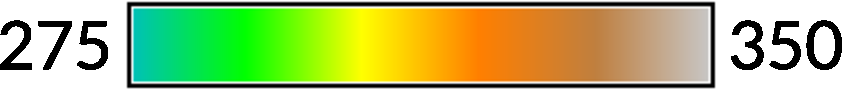
\includegraphics[width=0.19\textwidth]{images/legends/elevation_legend_1.pdf} & 
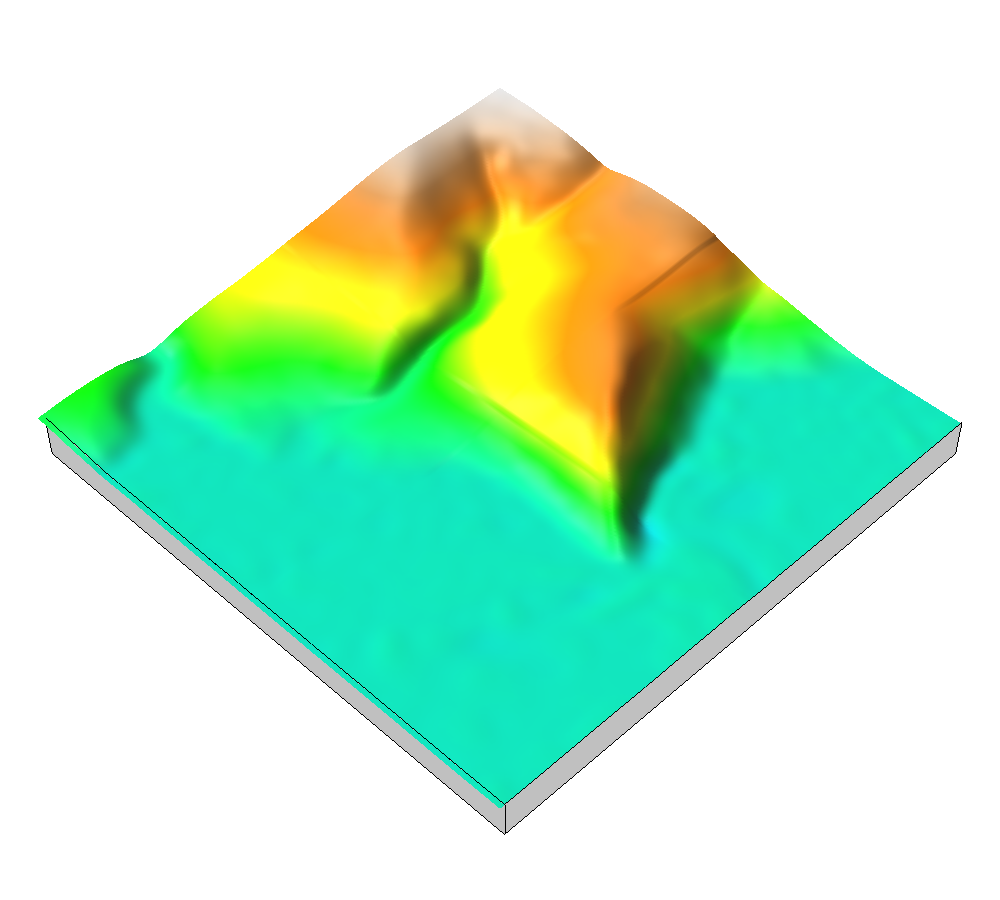
\includegraphics[width=0.19\textwidth]{images/render_3d/dem_1.png} &
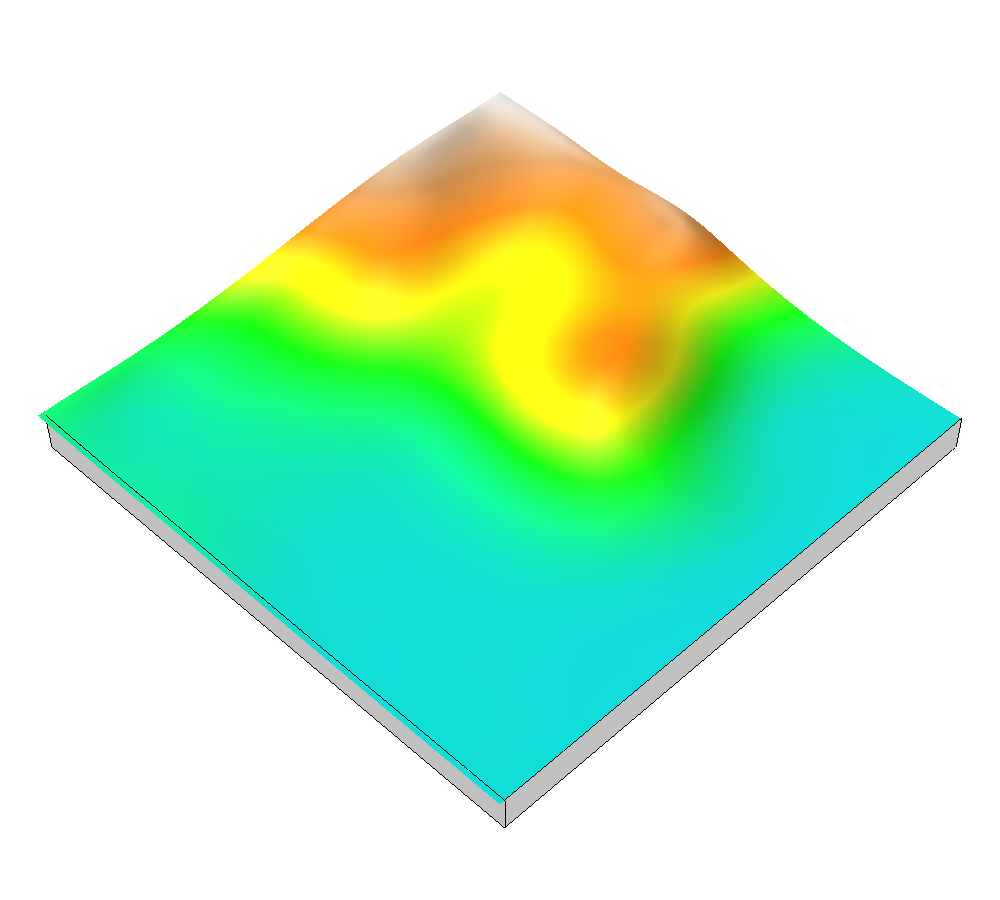
\includegraphics[width=0.19\textwidth]{images/render_3d/mean_dem_1.png} &
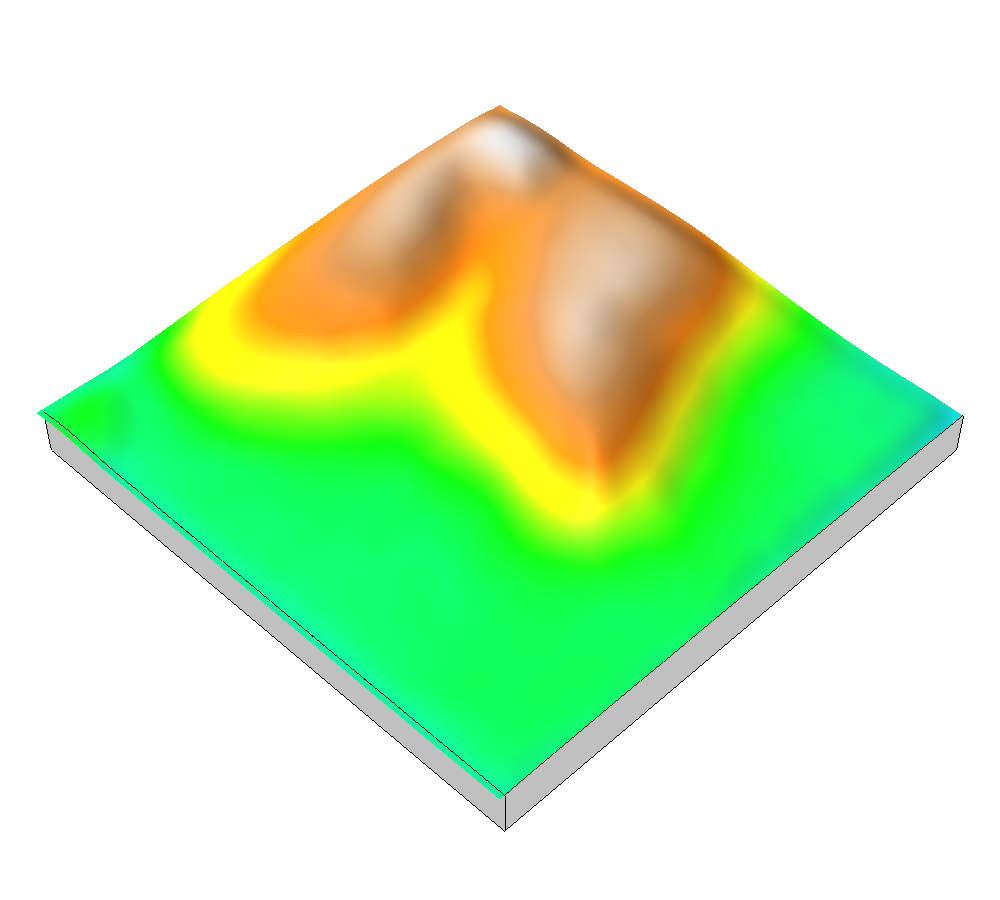
\includegraphics[width=0.19\textwidth]{images/render_3d/mean_dem_2.png} &
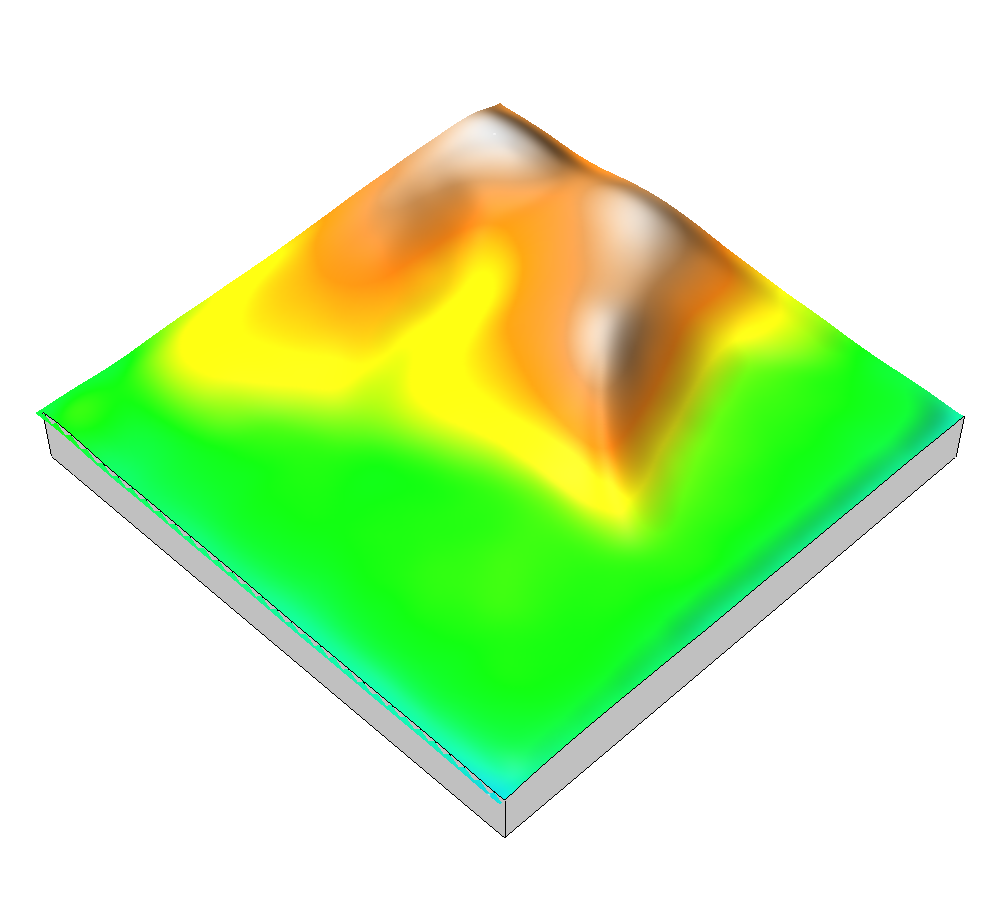
\includegraphics[width=0.19\textwidth]{images/render_3d/mean_dem_3.png}\\
%
Stdev.~of elevations \par \vspace{0.5em} 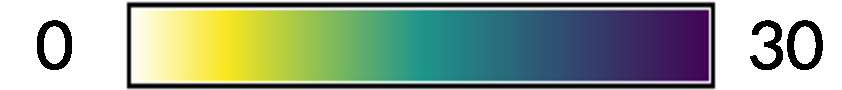
\includegraphics[width=0.19\textwidth]{images/legends/stdev_legend.pdf} & 
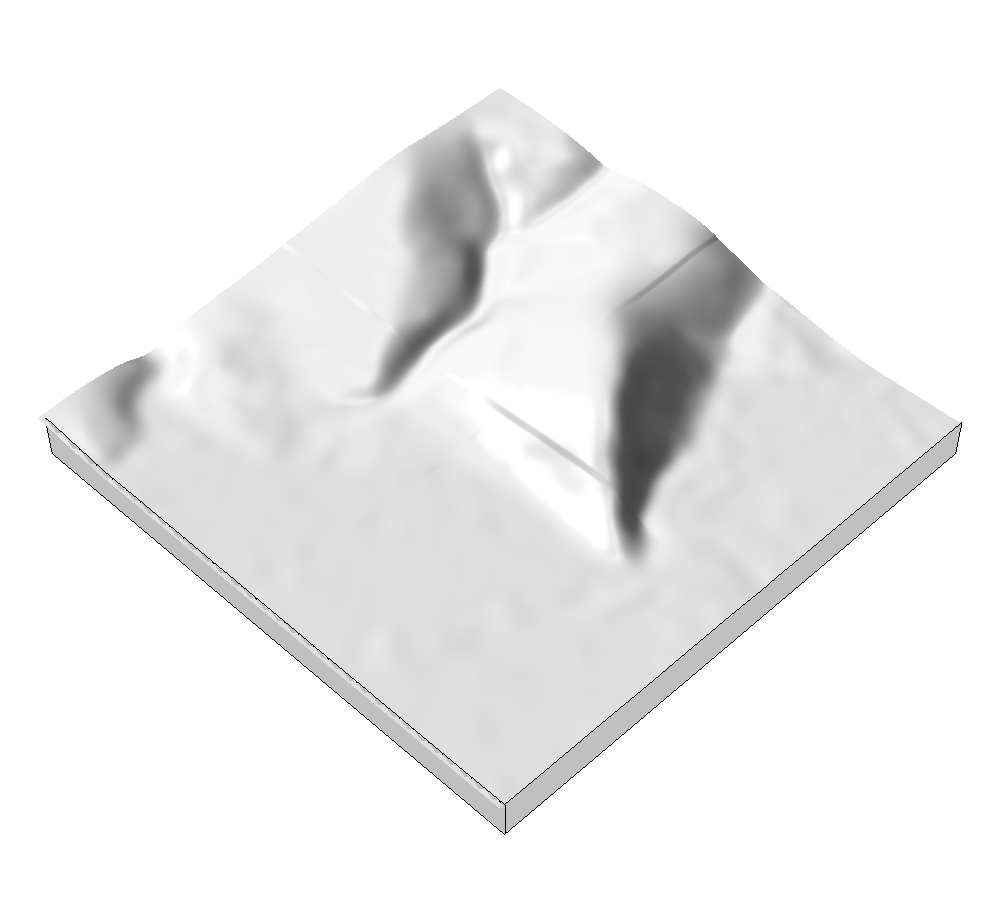
\includegraphics[width=0.19\textwidth]{images/render_3d/dem_difference_1.png} &
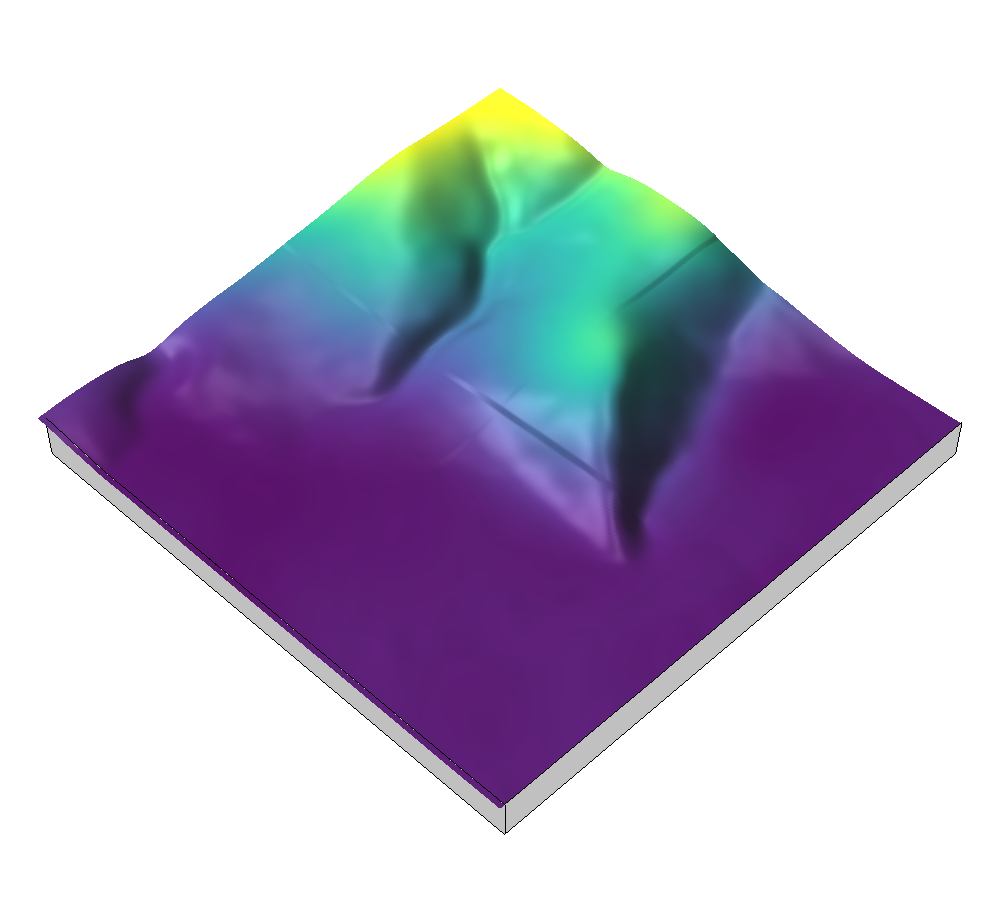
\includegraphics[width=0.19\textwidth]{images/render_3d/stdev_dem_1.png} &
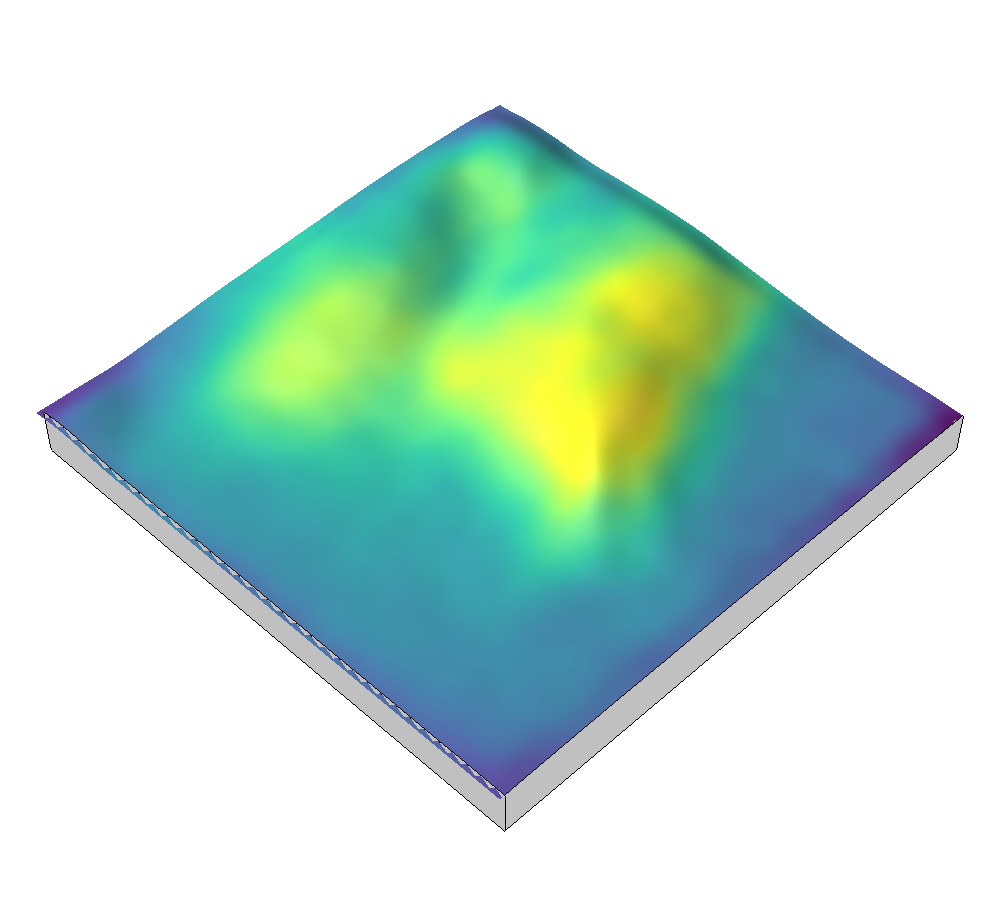
\includegraphics[width=0.19\textwidth]{images/render_3d/stdev_dem_2.png} &
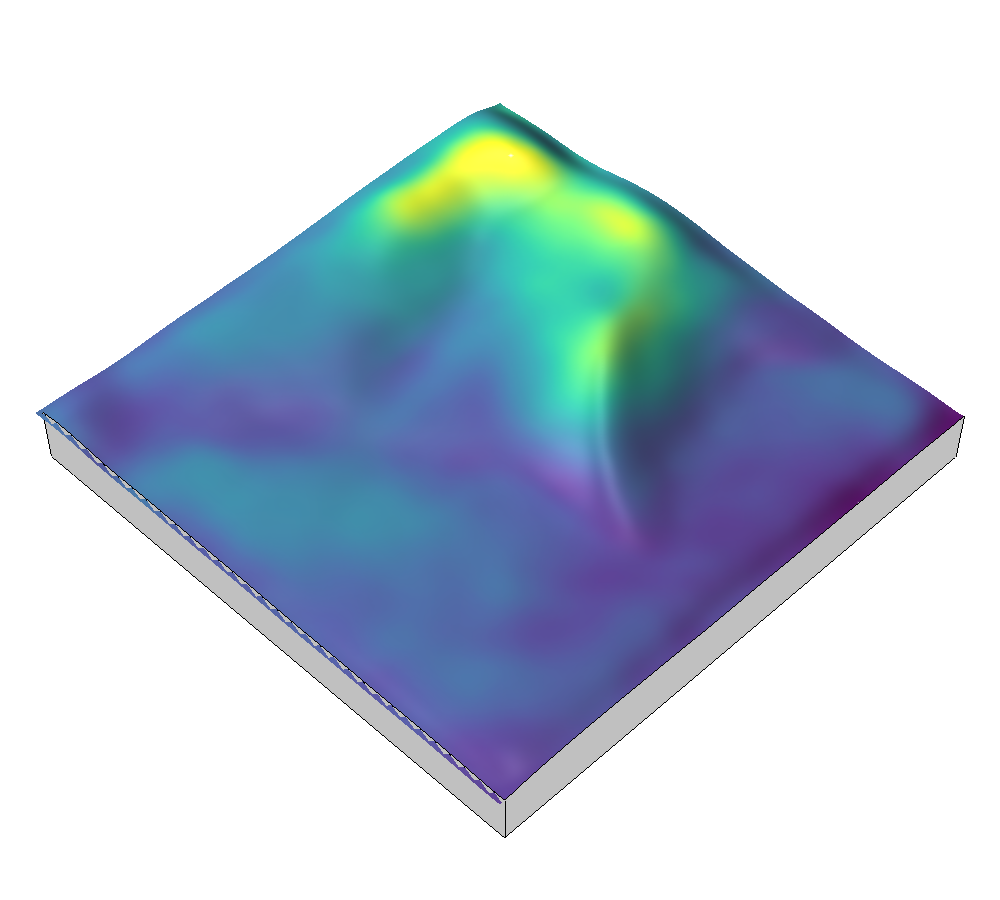
\includegraphics[width=0.19\textwidth]{images/render_3d/stdev_dem_3.png}\\
%
Stdev.~of difference \par \vspace{0.5em} 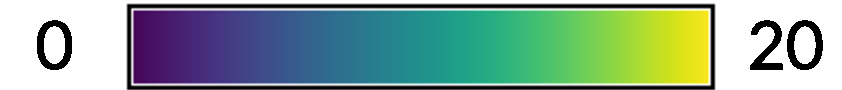
\includegraphics[width=0.19\textwidth]{images/legends/stdev_diff_legend.pdf} & 
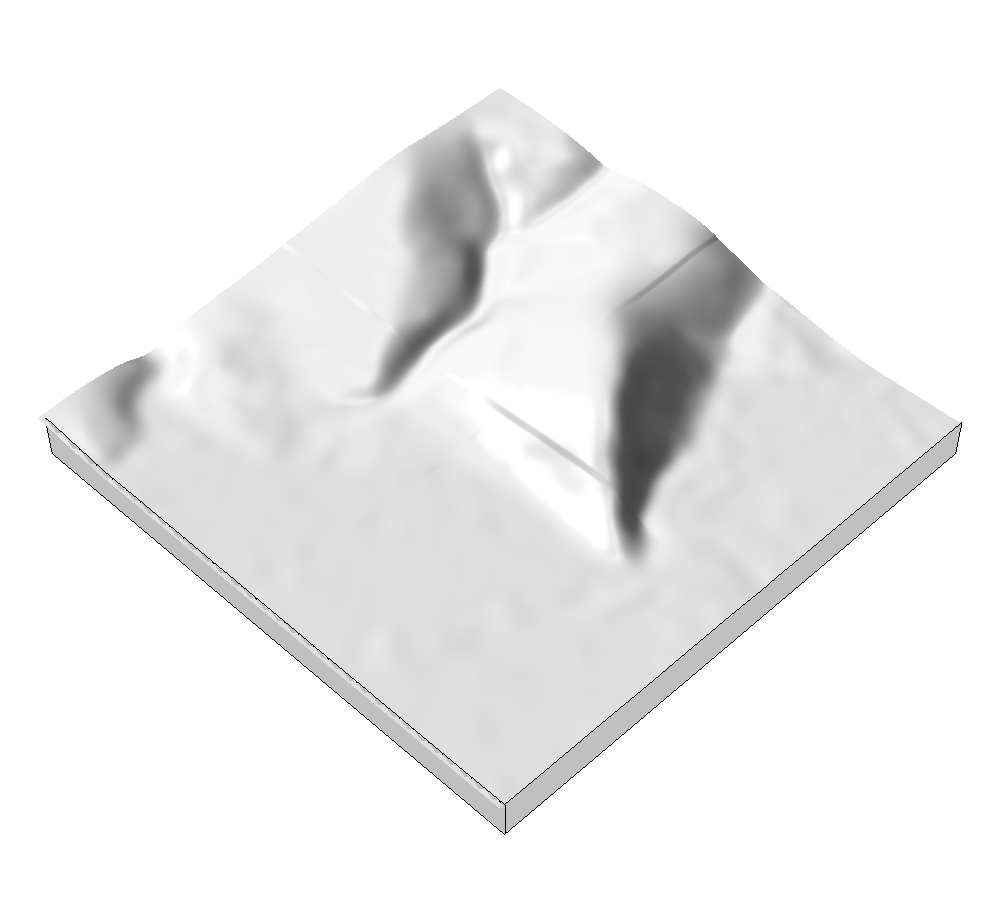
\includegraphics[width=0.19\textwidth]{images/render_3d/dem_difference_1.png} &
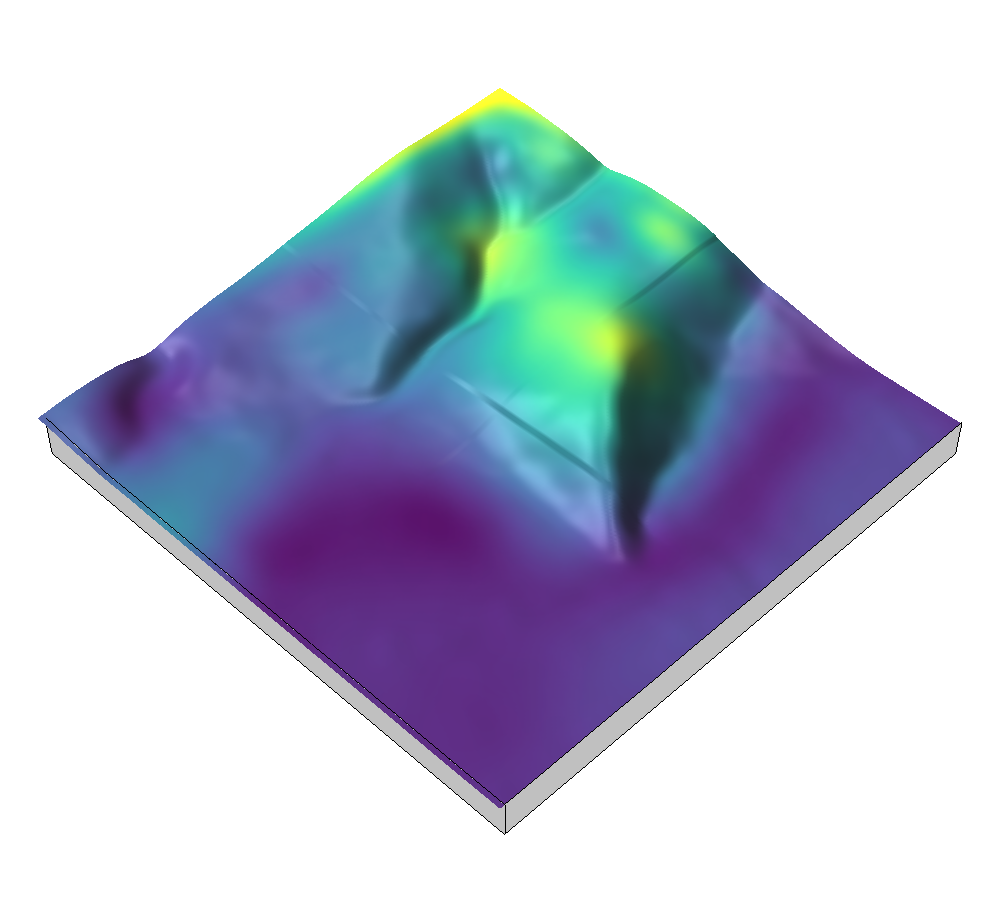
\includegraphics[width=0.19\textwidth]{images/render_3d/stdev_regression_difference_series_1.png} &
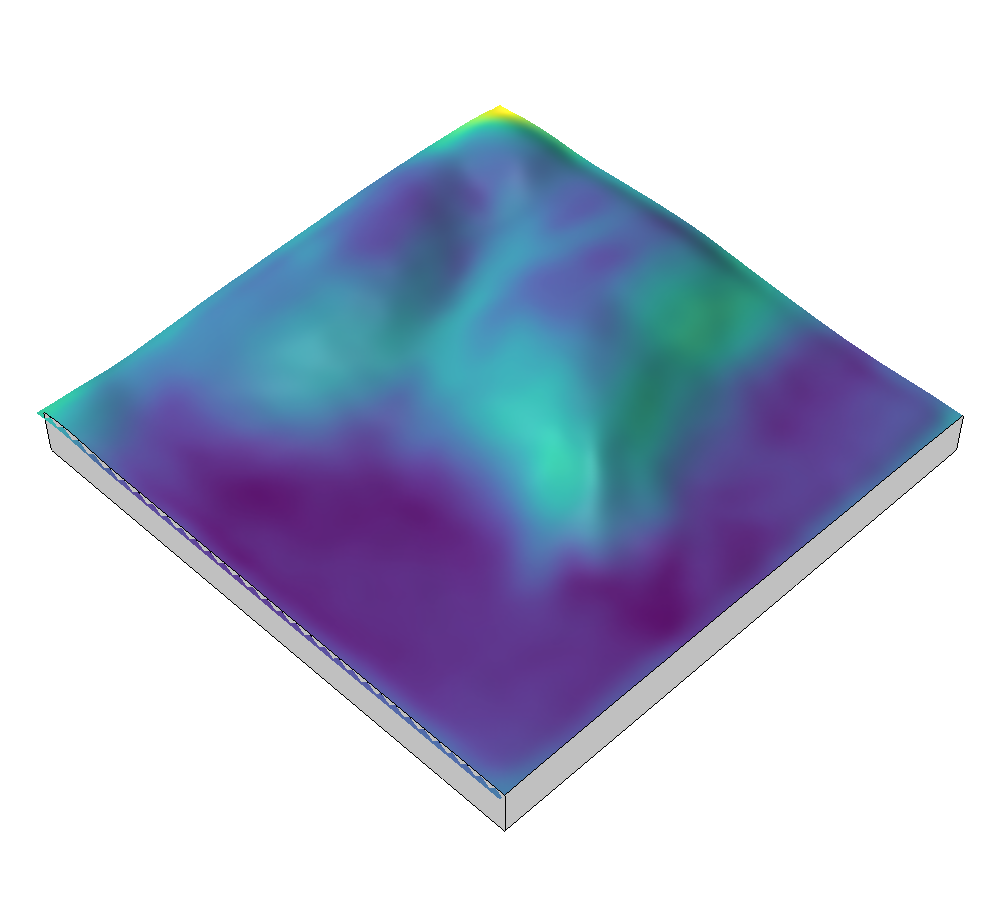
\includegraphics[width=0.19\textwidth]{images/render_3d/stdev_regression_difference_series_2.png} &
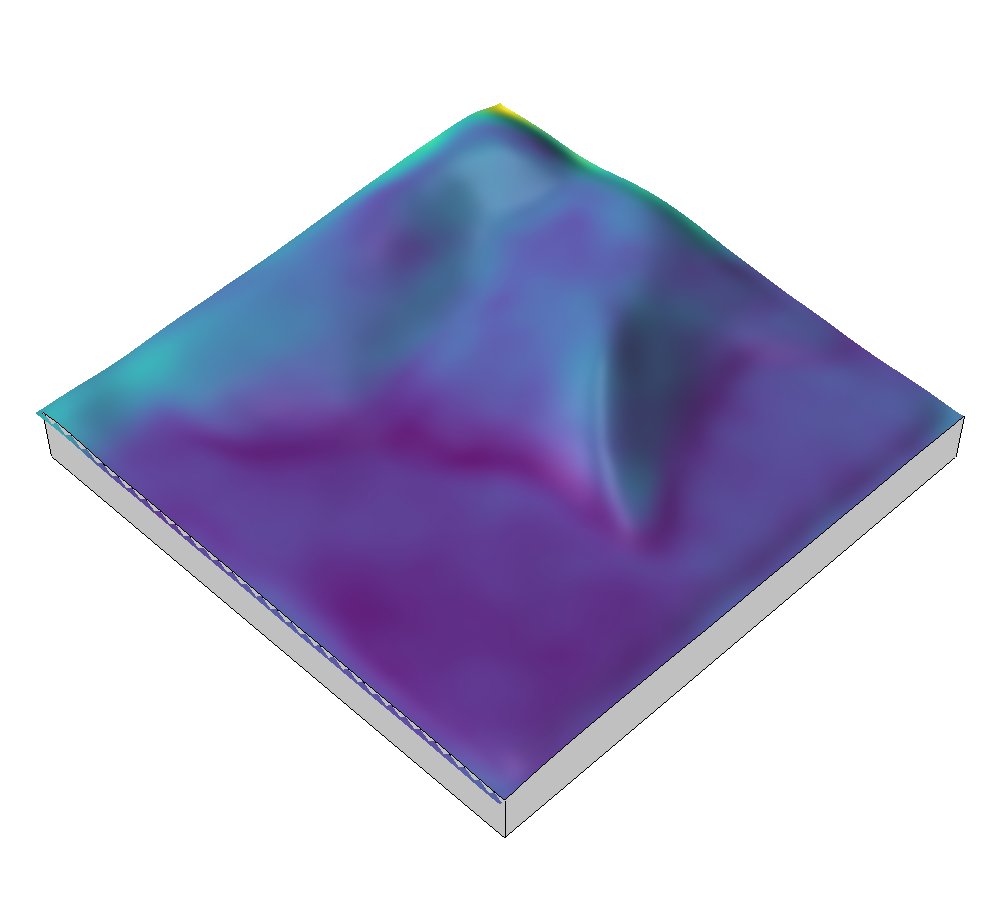
\includegraphics[width=0.19\textwidth]{images/render_3d/stdev_regression_difference_series_3.png}\\
%
Mean difference \par \vspace{0.5em} 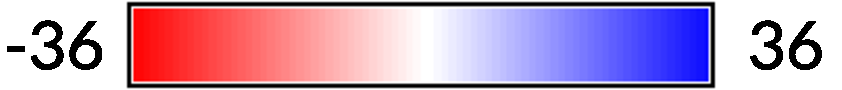
\includegraphics[width=0.19\textwidth]{images/legends/diff_legend.pdf} & 
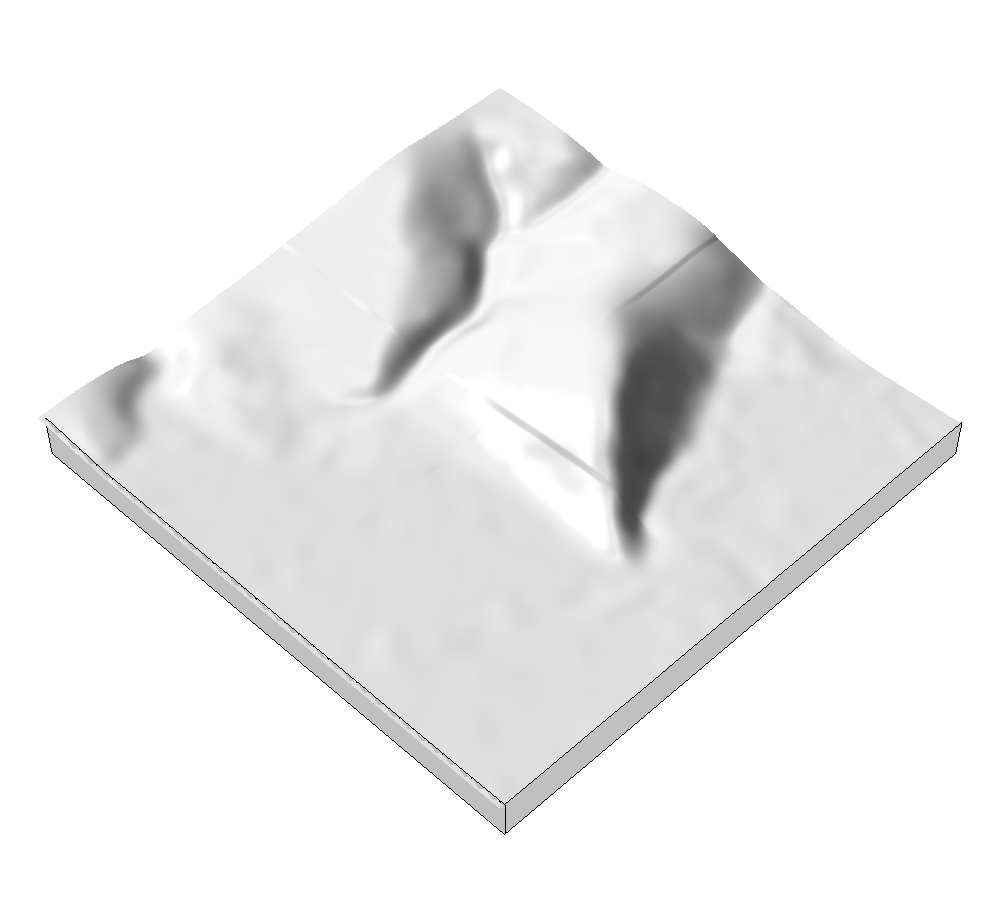
\includegraphics[width=0.19\textwidth]{images/render_3d/dem_difference_1.png} &
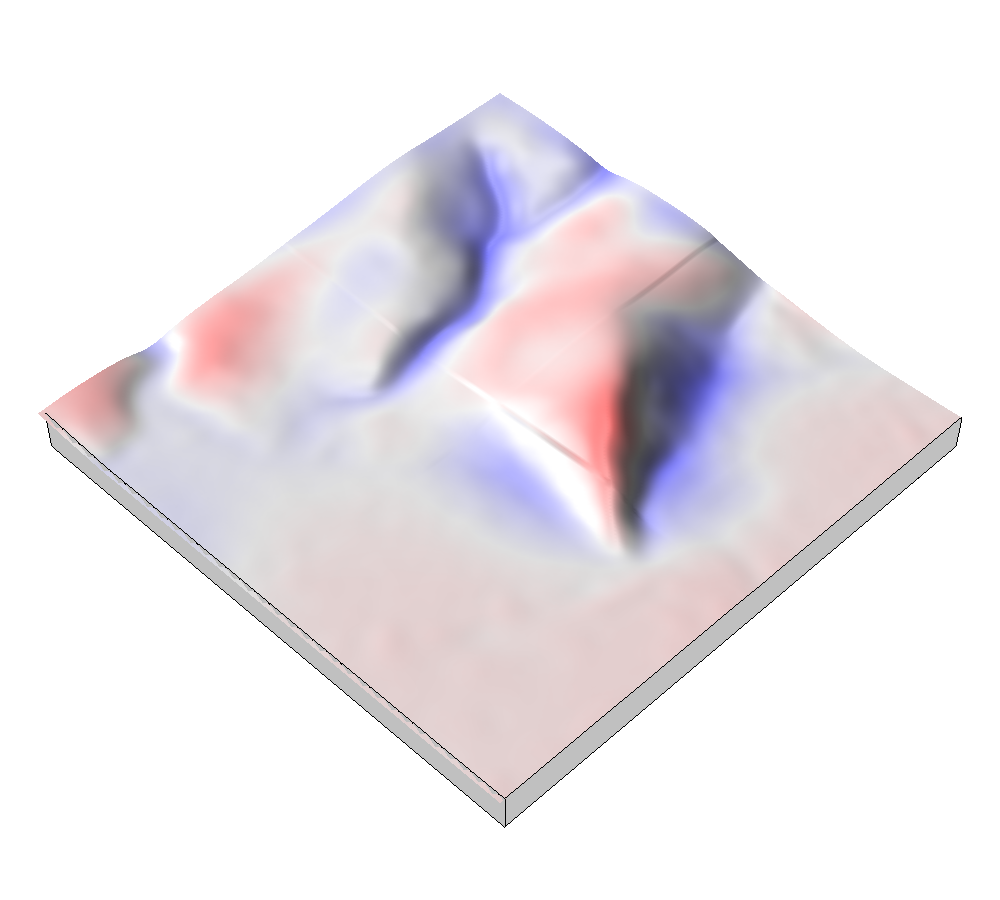
\includegraphics[width=0.19\textwidth]{images/render_3d/mean_dem_regression_difference_1.png} &
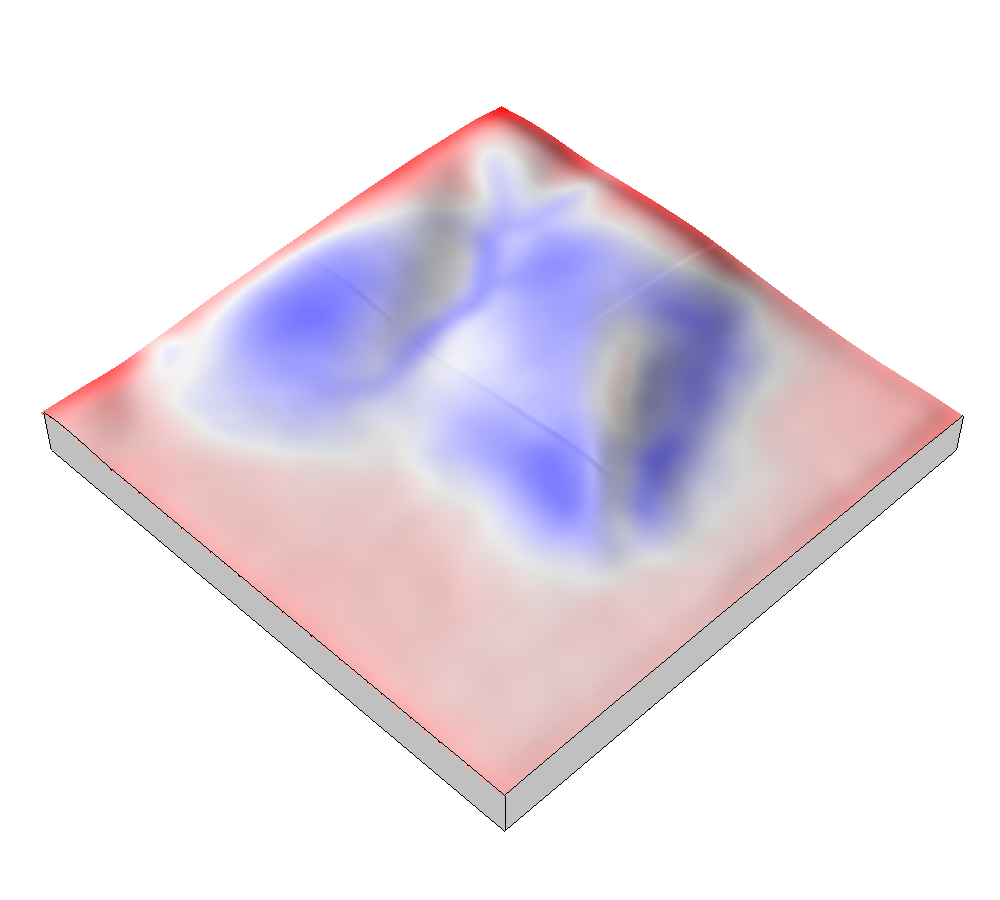
\includegraphics[width=0.19\textwidth]{images/render_3d/mean_dem_regression_difference_2.png} &
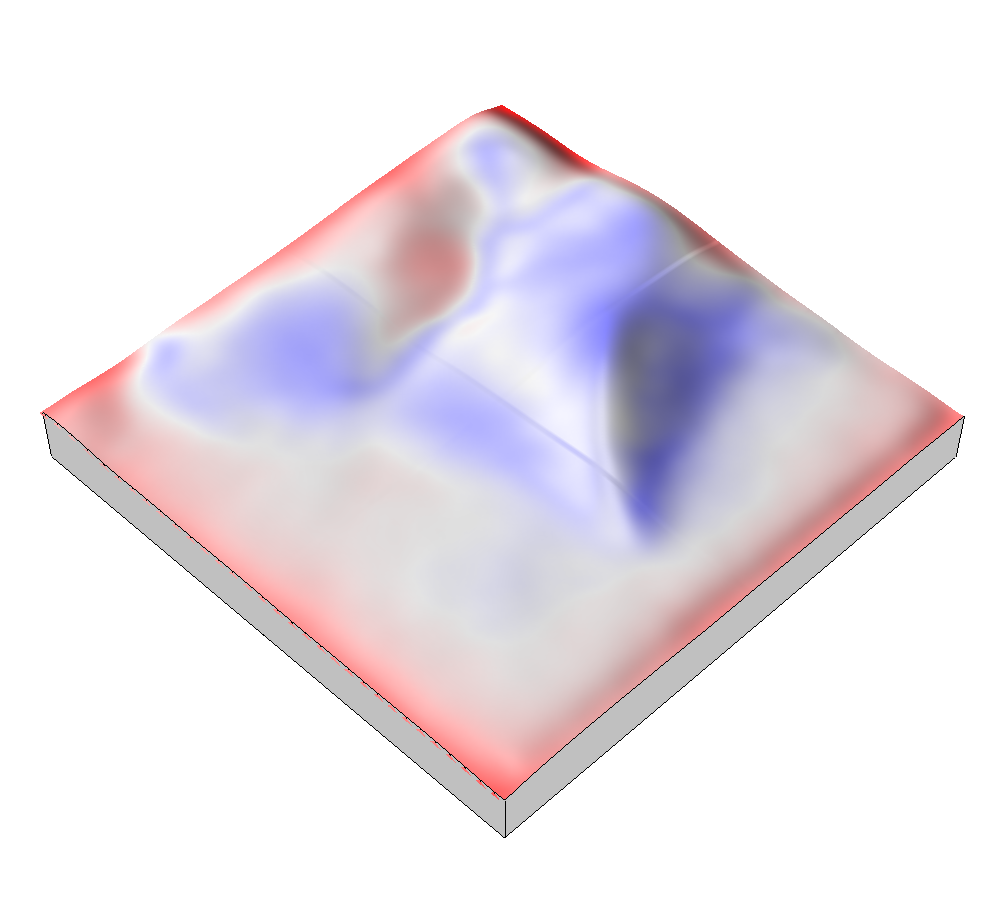
\includegraphics[width=0.19\textwidth]{images/render_3d/mean_dem_regression_difference_3.png}\\
%
Mean slope \par \vspace{0.5em} 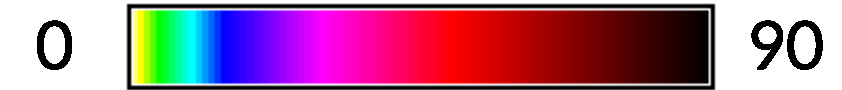
\includegraphics[width=0.19\textwidth]{images/legends/slope_legend.pdf} & 
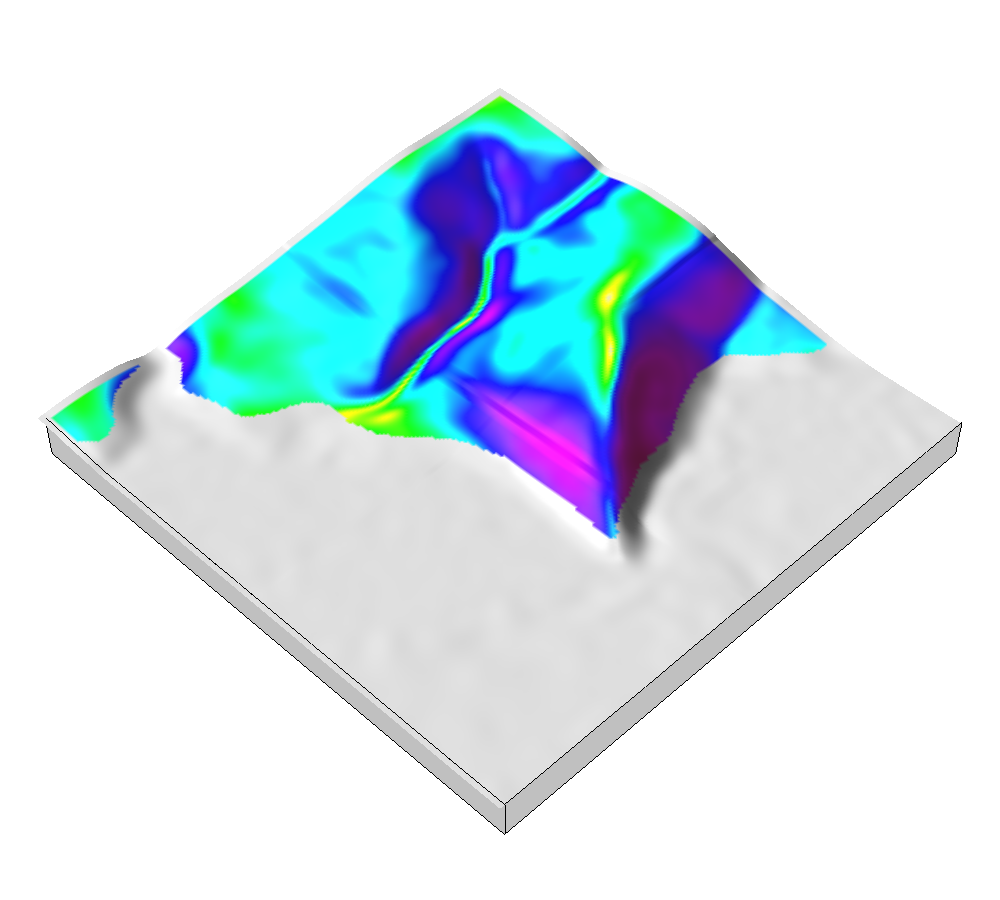
\includegraphics[width=0.19\textwidth]{images/render_3d/slope_1.png} &
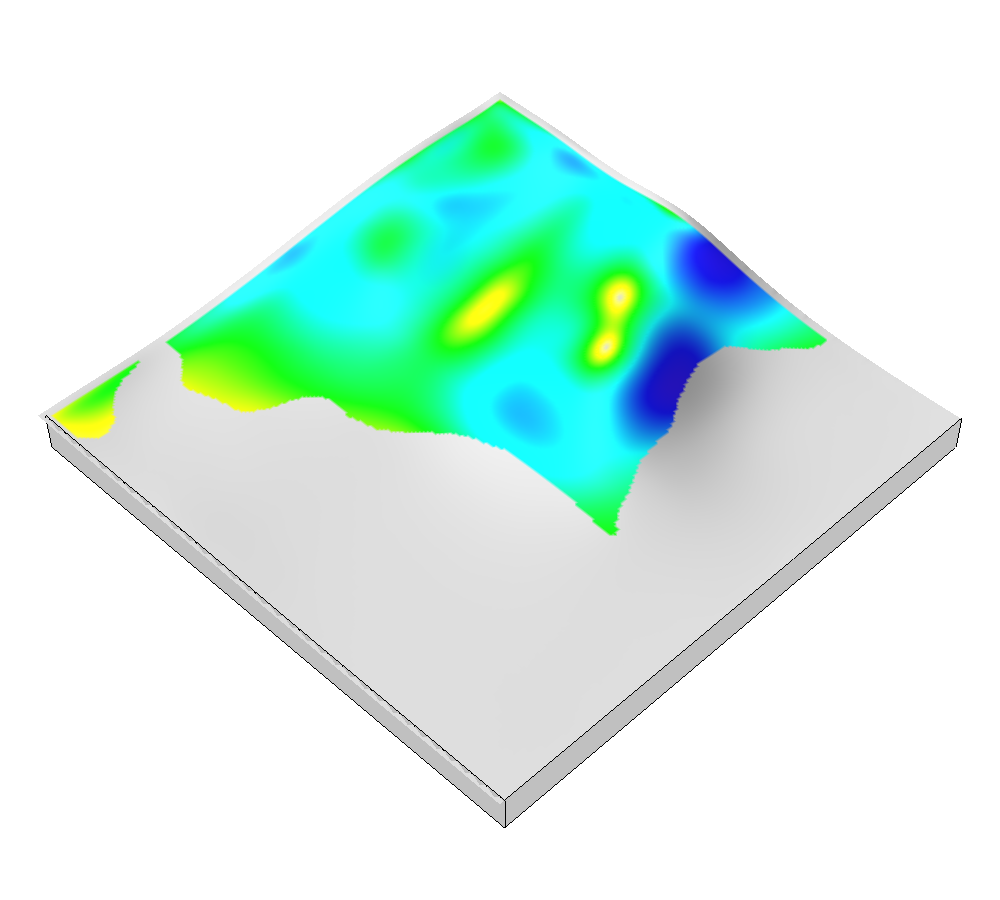
\includegraphics[width=0.19\textwidth]{images/render_3d/mean_slope_1.png} &
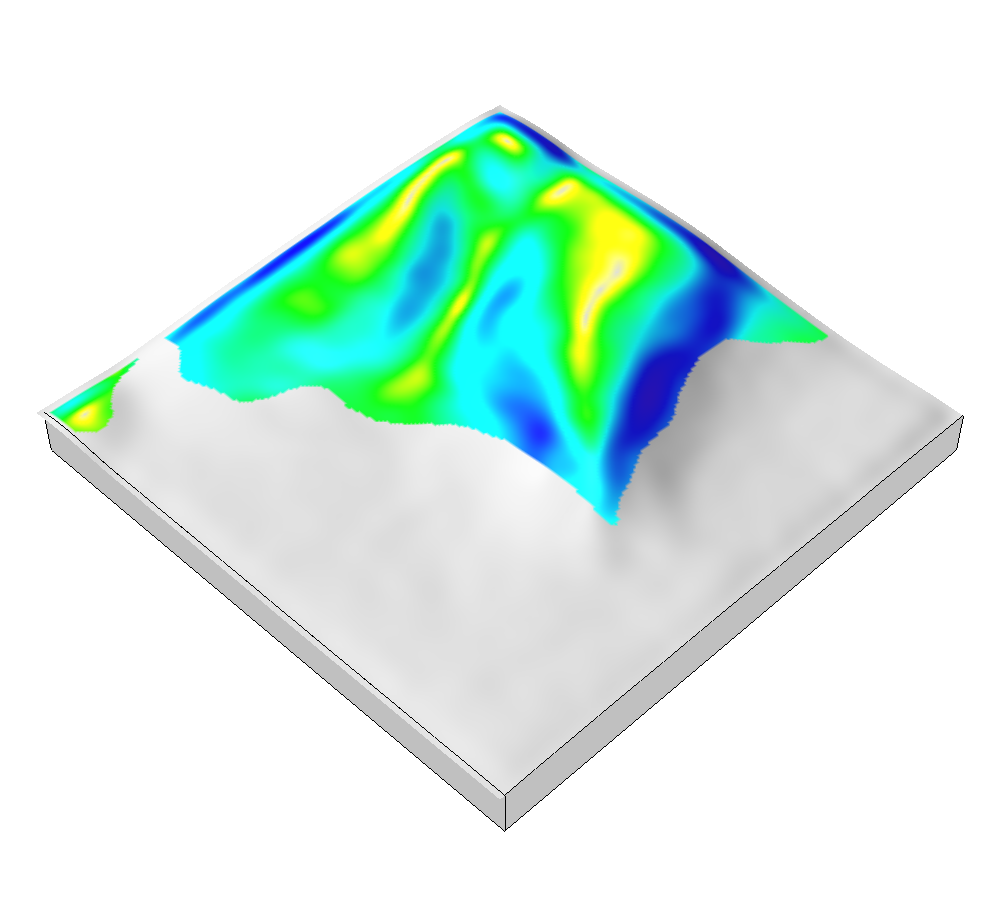
\includegraphics[width=0.19\textwidth]{images/render_3d/mean_slope_2.png} &
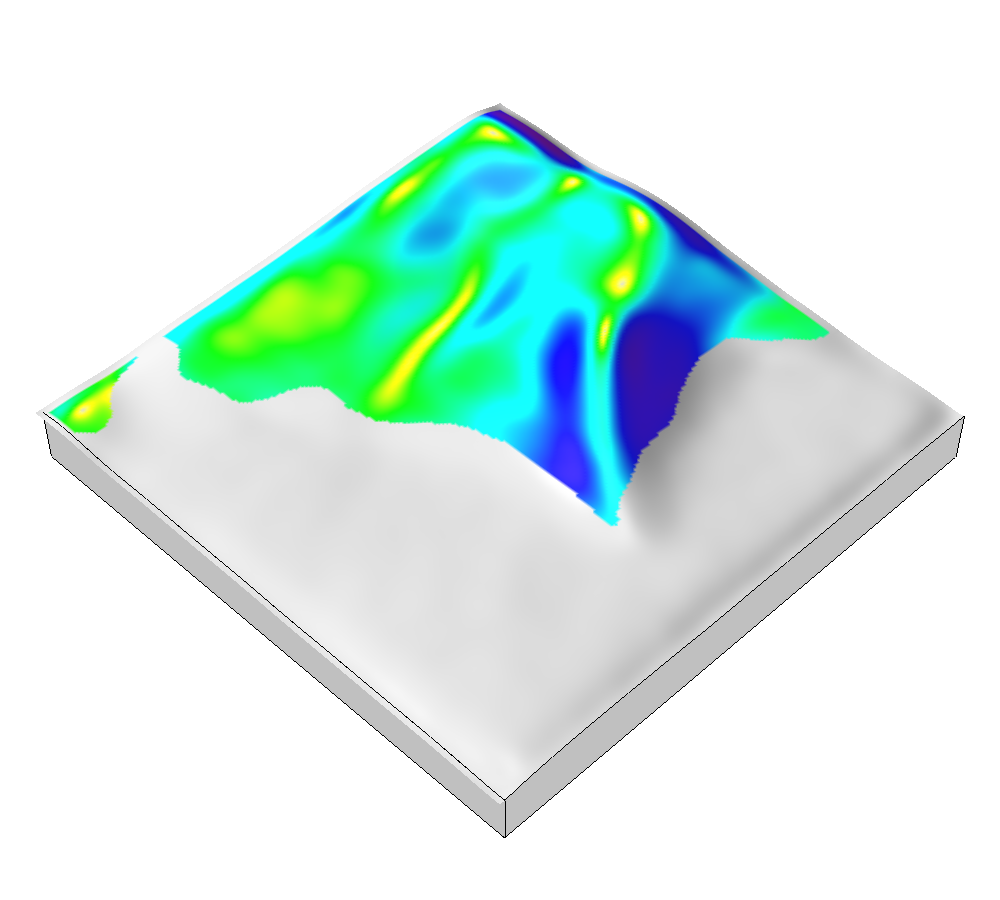
\includegraphics[width=0.19\textwidth]{images/render_3d/mean_slope_3.png}\\
%
Mean landforms \par \vspace{0.5em} 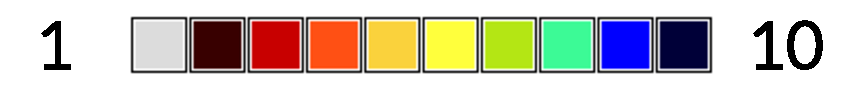
\includegraphics[width=0.19\textwidth]{images/legends/forms_legend.pdf} & 
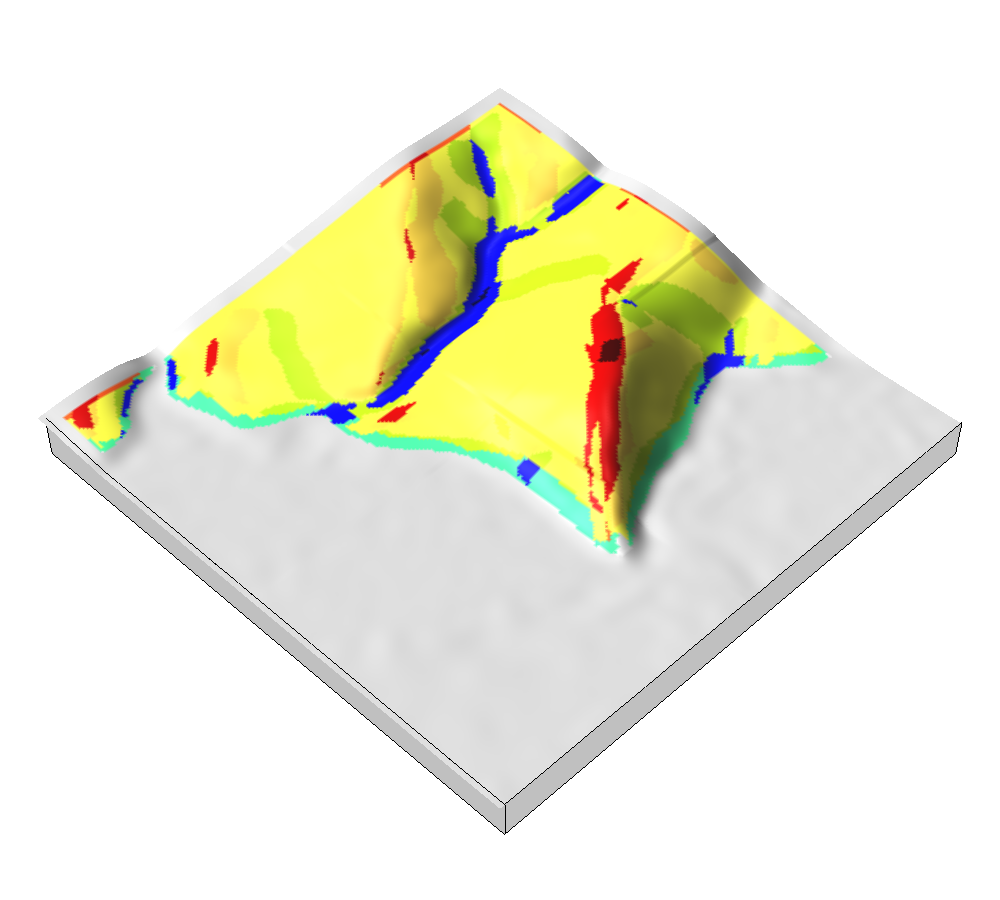
\includegraphics[width=0.19\textwidth]{images/render_3d/forms_1.png} &
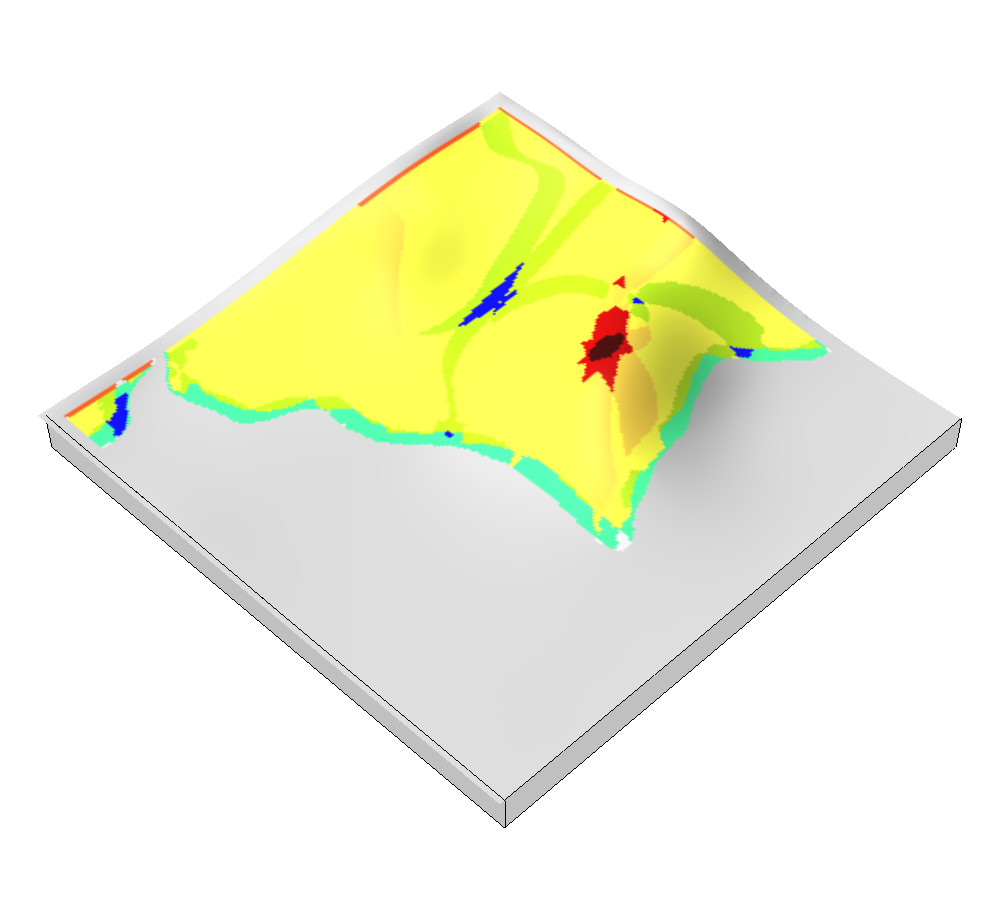
\includegraphics[width=0.19\textwidth]{images/render_3d/mean_forms_1.png} &
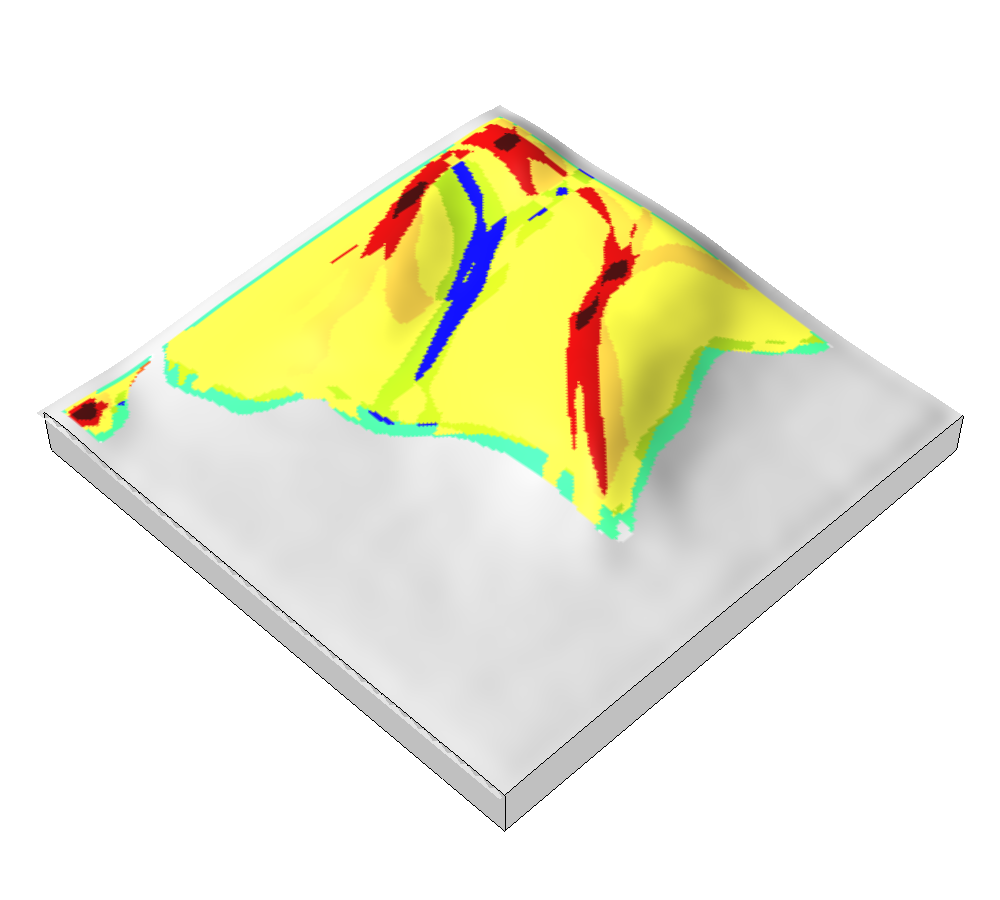
\includegraphics[width=0.19\textwidth]{images/render_3d/mean_forms_2.png} &
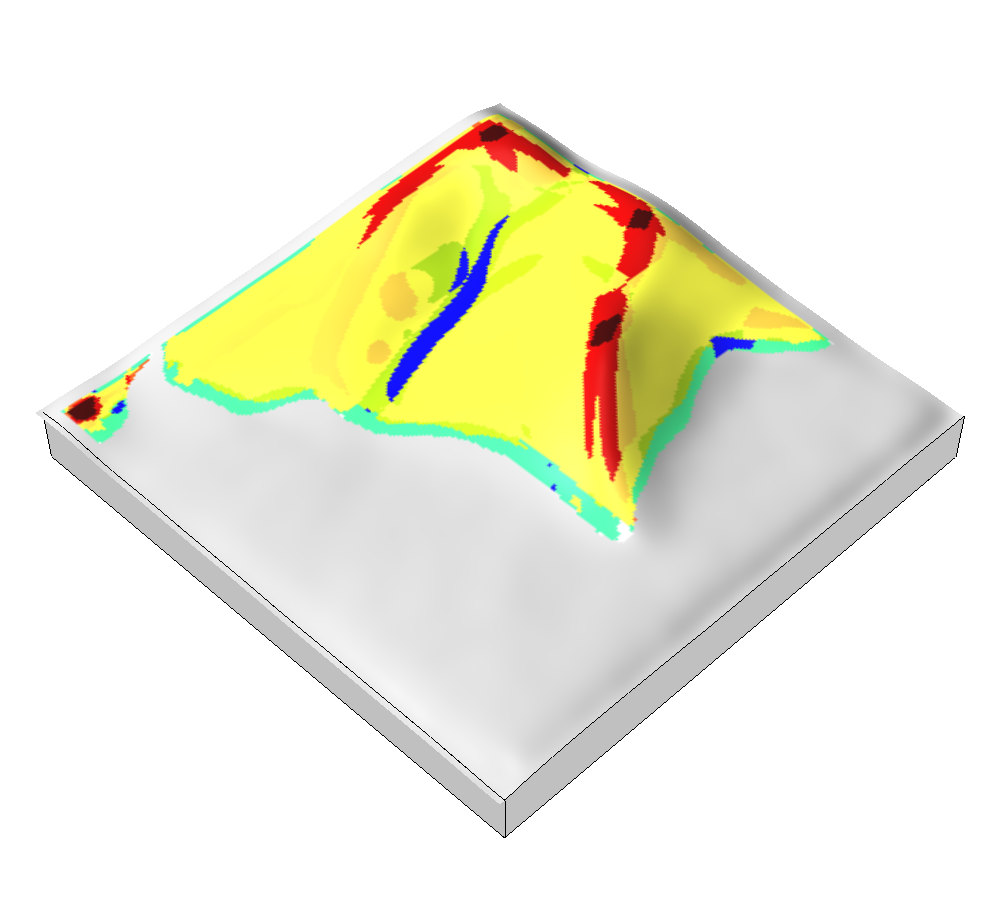
\includegraphics[width=0.19\textwidth]{images/render_3d/mean_forms_3.png}\\
%
\bottomrule
\end{tabular}}
\label{table:coupling_experiment} 
\end{table}
%

%%%%%%%%%%%%%%%%%%   DIFFERENCE STATS TABLE

\begin{table}
\tbl{Difference experiment}{
\ra{1.3}
\begin{tabular}{m{0.24\textwidth} m{0.24\textwidth} m{0.24\textwidth} m{0.24\textwidth}}
\toprule
\multicolumn{1}{c}{Reference elevation} & \multicolumn{1}{c}{Mean elevation} & \multicolumn{1}{c}{Stdev.~ of elevations}  & \multicolumn{1}{c}{Stdev.~ of differences}\\
\midrule
%
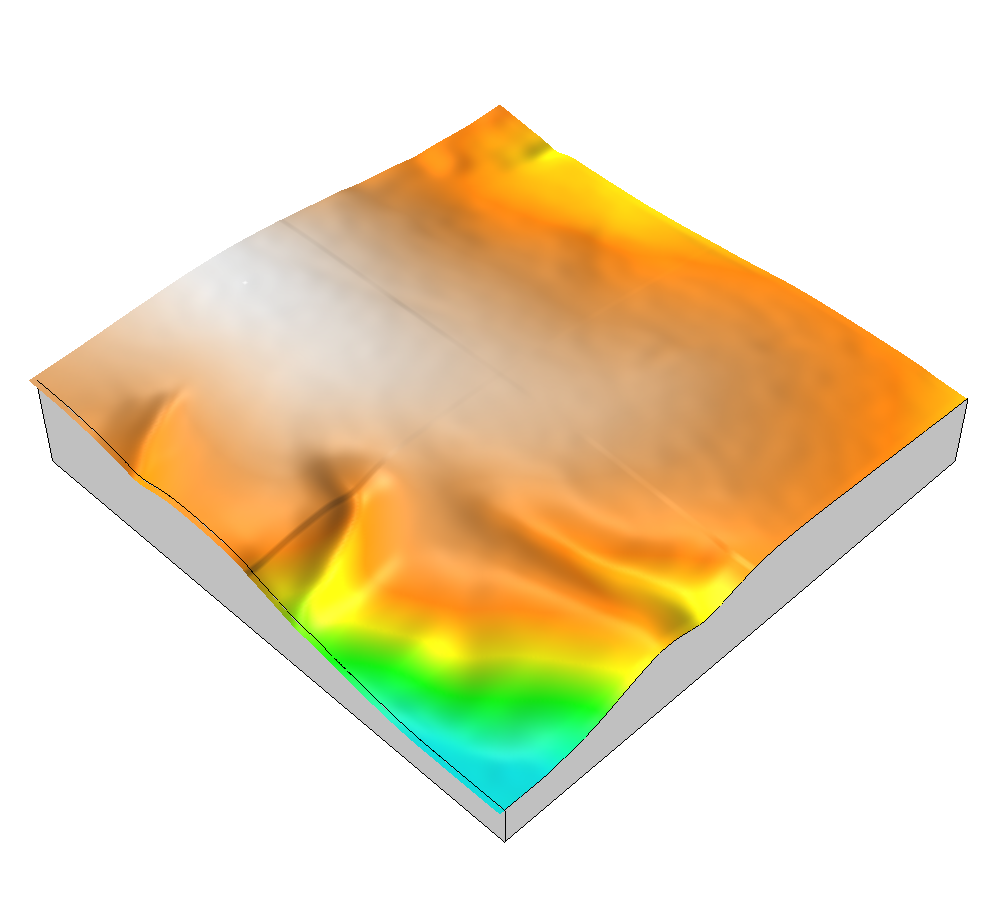
\includegraphics[width=0.24\textwidth]{images/render_3d/dem_4.png} &
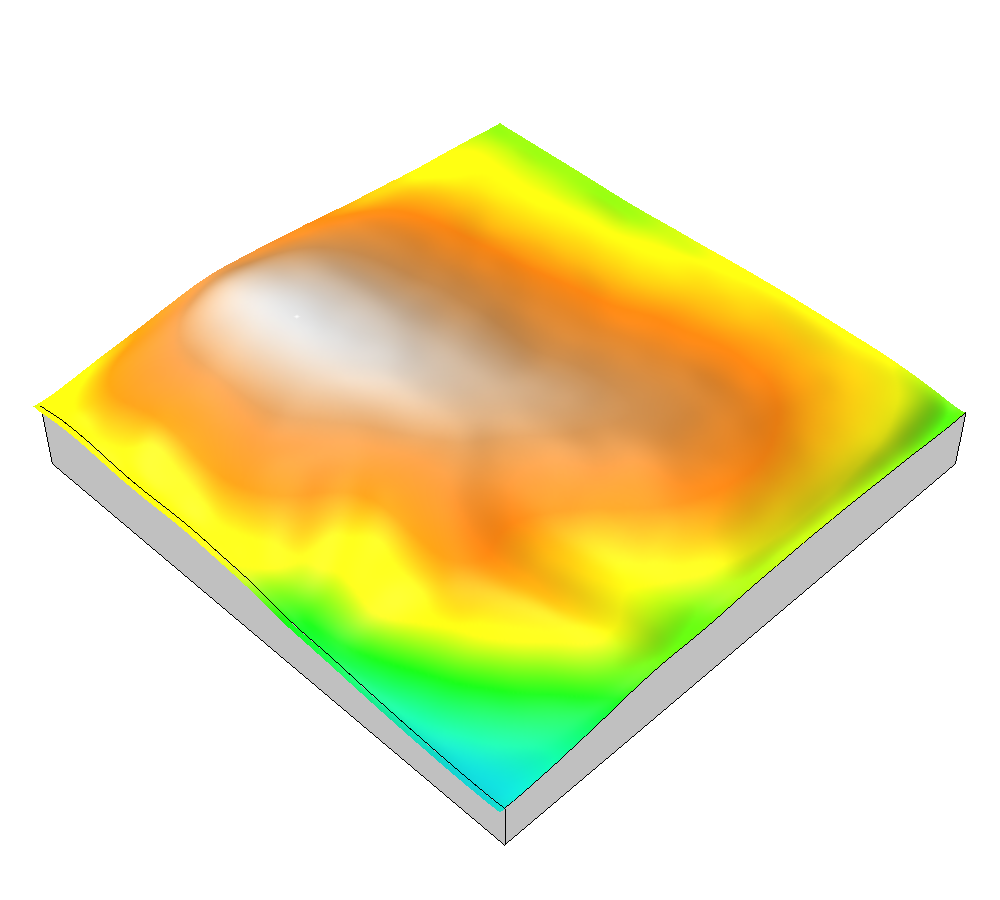
\includegraphics[width=0.24\textwidth]{images/render_3d/mean_dem_4.png} &
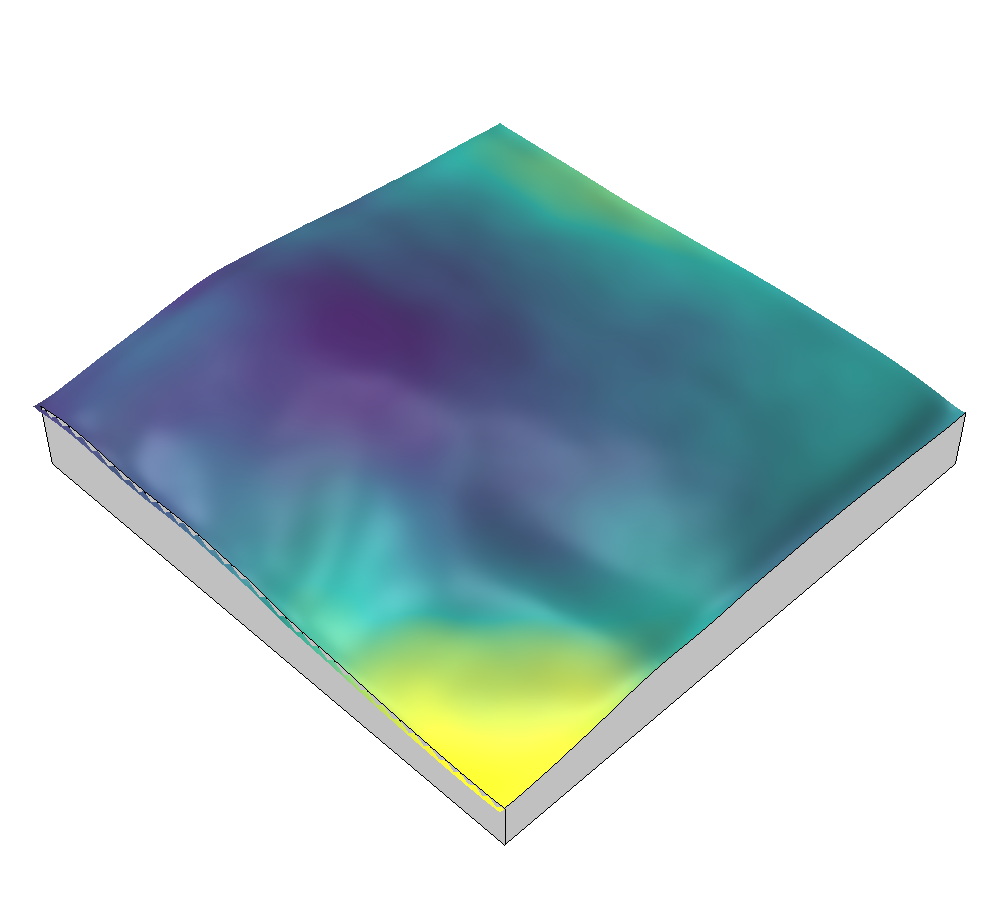
\includegraphics[width=0.24\textwidth]{images/render_3d/stdev_dem_4.png} &
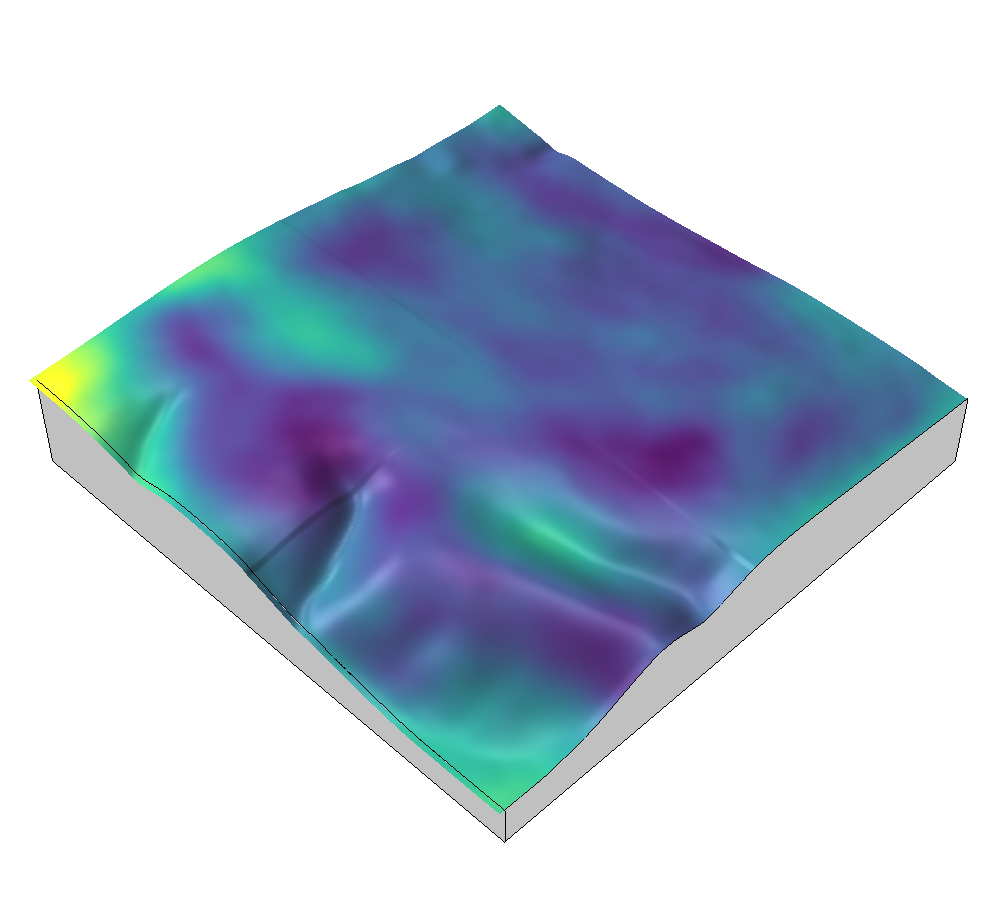
\includegraphics[width=0.24\textwidth]{images/render_3d/stdev_regression_difference_series_4.png}\\
%
\multicolumn{1}{c}{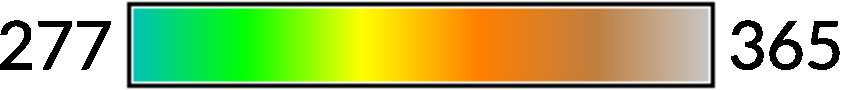
\includegraphics[width=0.22\textwidth]{images/legends/elevation_legend_4.pdf}} &
\multicolumn{1}{c}{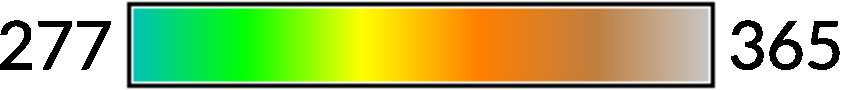
\includegraphics[width=0.22\textwidth]{images/legends/elevation_legend_4.pdf}} &
\multicolumn{1}{c}{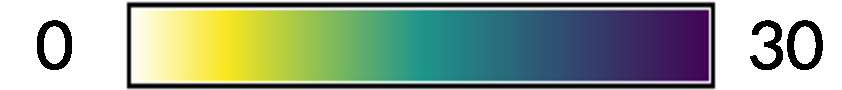
\includegraphics[width=0.22\textwidth]{images/legends/stdev_legend.pdf}} &
\multicolumn{1}{c}{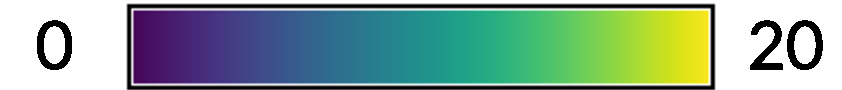
\includegraphics[width=0.22\textwidth]{images/legends/stdev_diff_legend.pdf}}\\
%
\bottomrule
\end{tabular}}
\label{table:difference_stats} 
\end{table}

%%%%%%%%%%%%%%%%%% DIFFERENCE TABLE

\begin{table}
\tbl{Difference experiment}{
\ra{1.3}
\begin{tabular}{m{0.1\textwidth} m{0.22\textwidth} m{0.22\textwidth} m{0.22\textwidth} m{0.22\textwidth}}
\toprule
& \multicolumn{1}{c}{Elevation} & \multicolumn{1}{c}{Elevation difference} & \multicolumn{1}{c}{Slope}  & \multicolumn{1}{c}{Landform}\\
\midrule
%
Reference & 
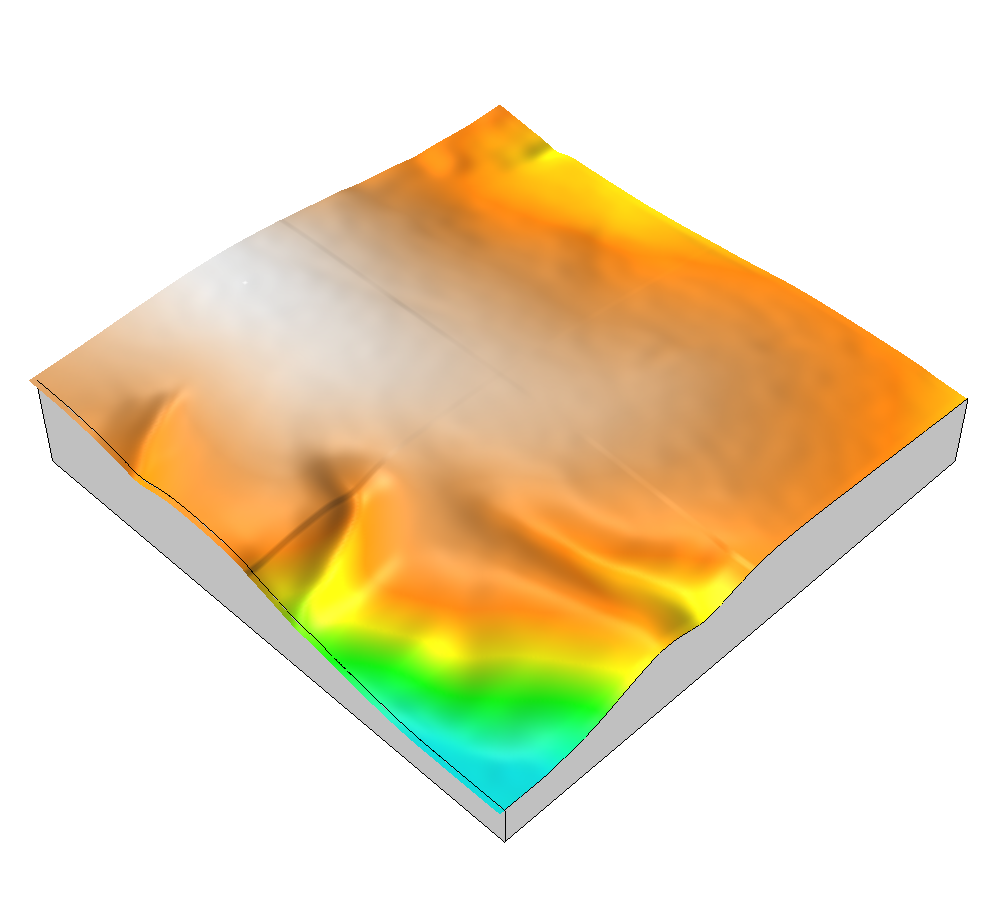
\includegraphics[width=0.22\textwidth]{images/render_3d/dem_4.png} &
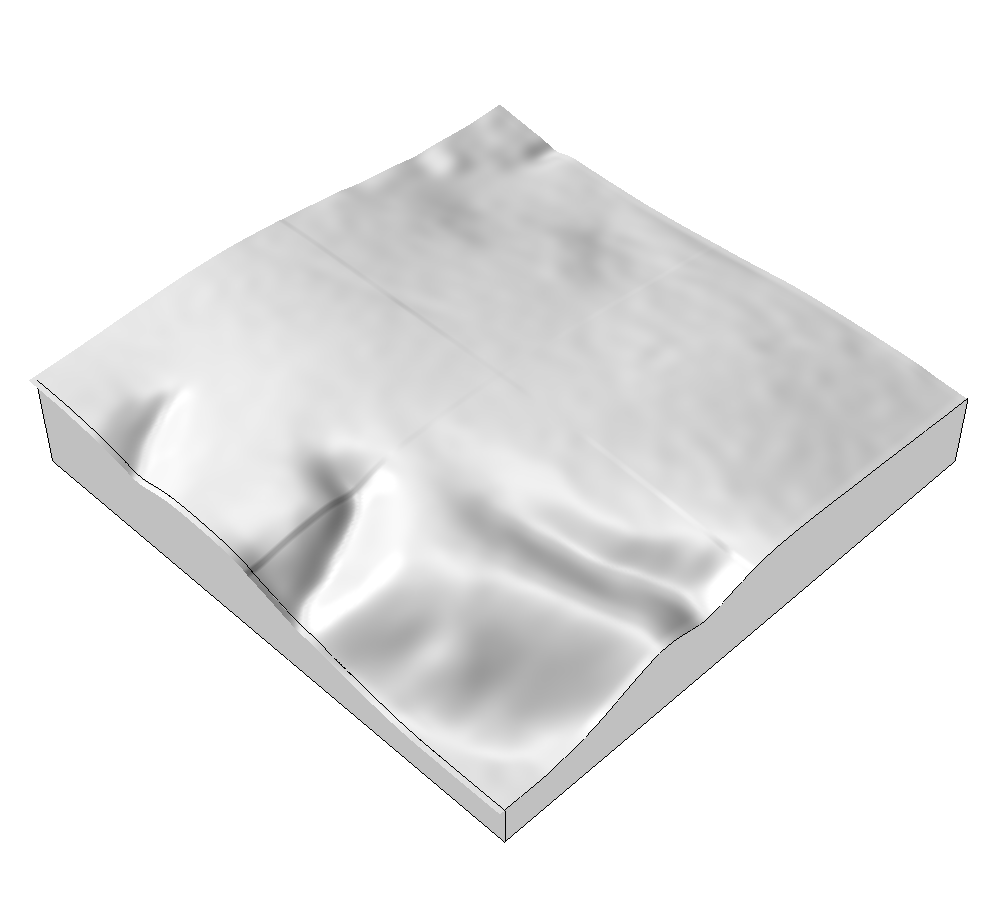
\includegraphics[width=0.22\textwidth]{images/render_3d/dem_difference_4.png} &
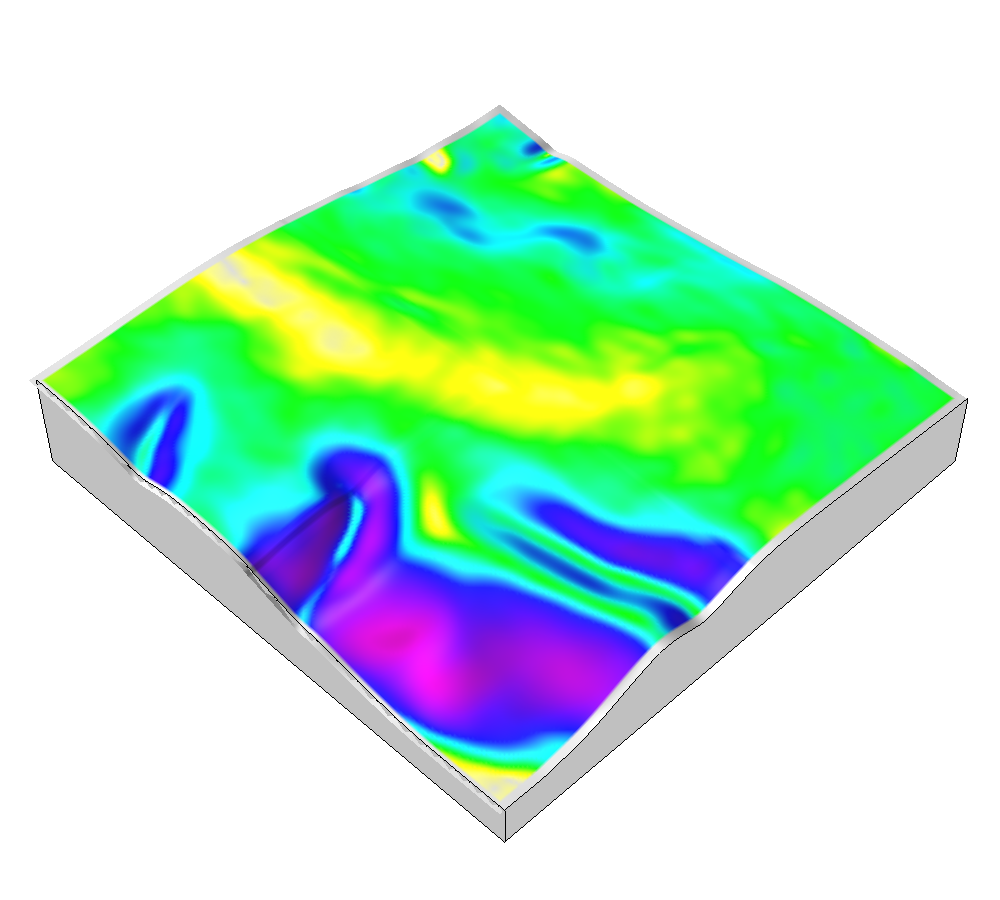
\includegraphics[width=0.22\textwidth]{images/render_3d/slope_4.png} &
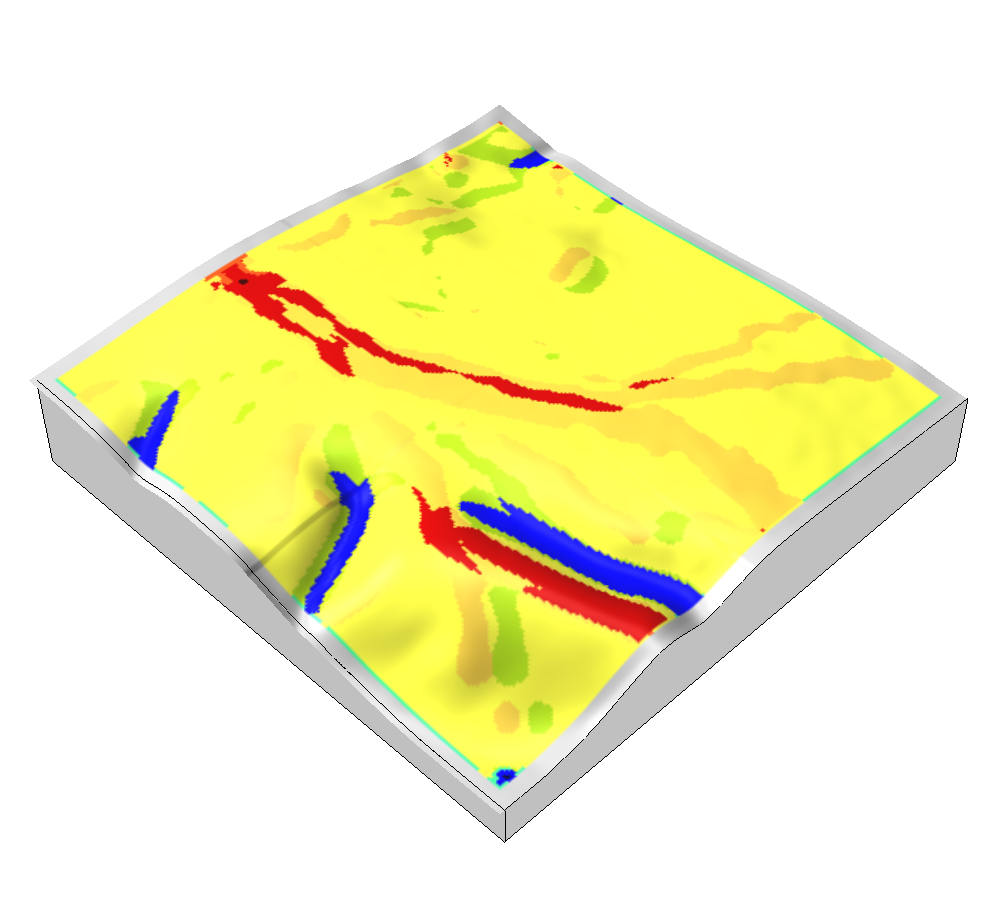
\includegraphics[width=0.22\textwidth]{images/render_3d/forms_4.png}\\
%
Mean & 
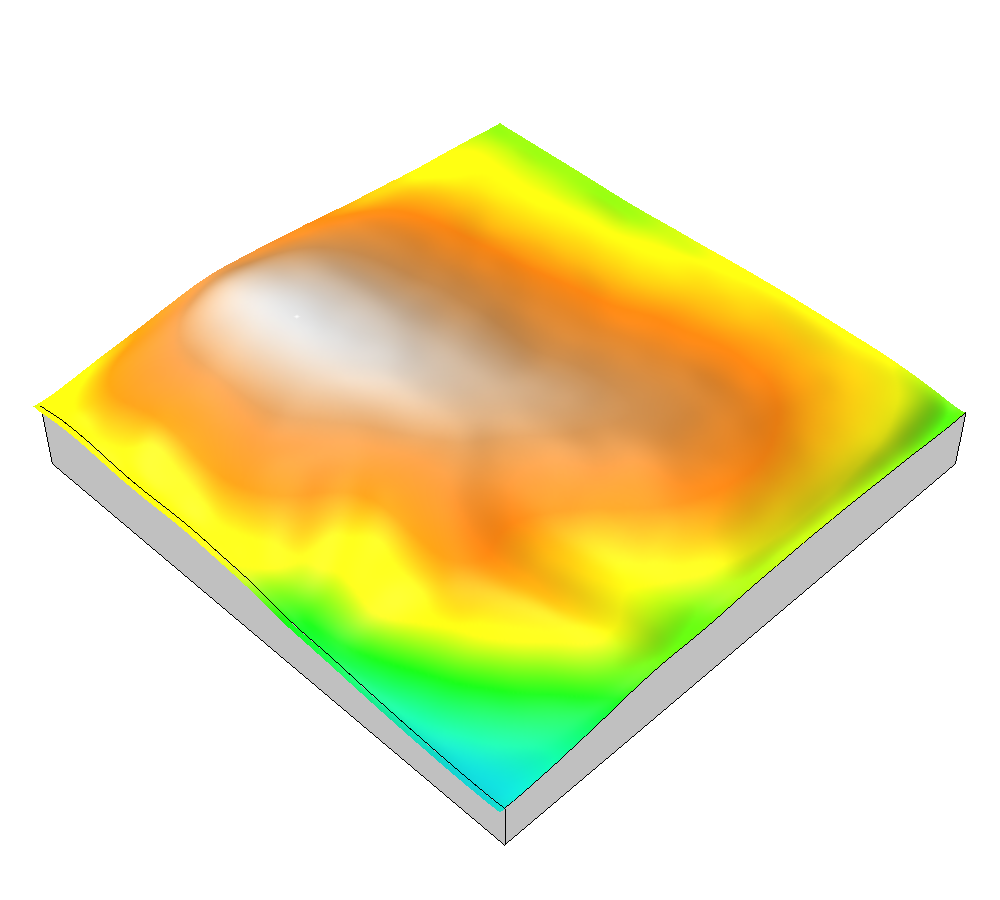
\includegraphics[width=0.22\textwidth]{images/render_3d/mean_dem_4.png} &
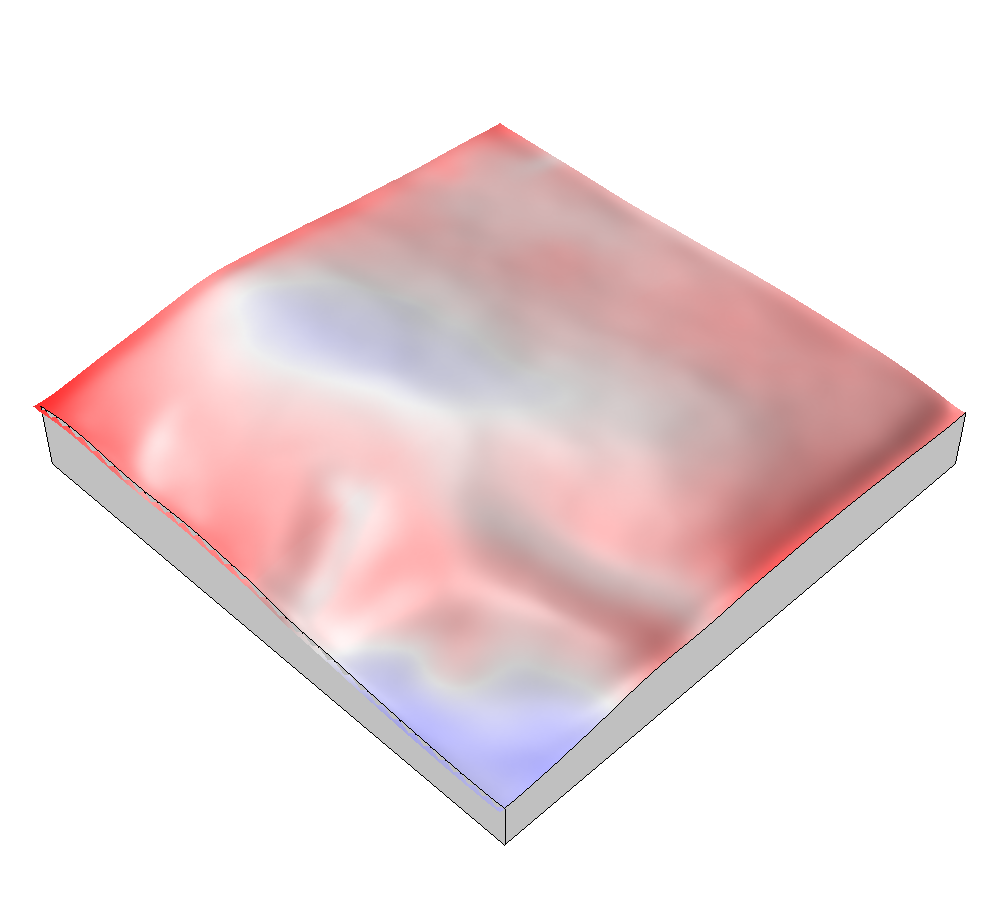
\includegraphics[width=0.22\textwidth]{images/render_3d/mean_dem_difference_4.png} &
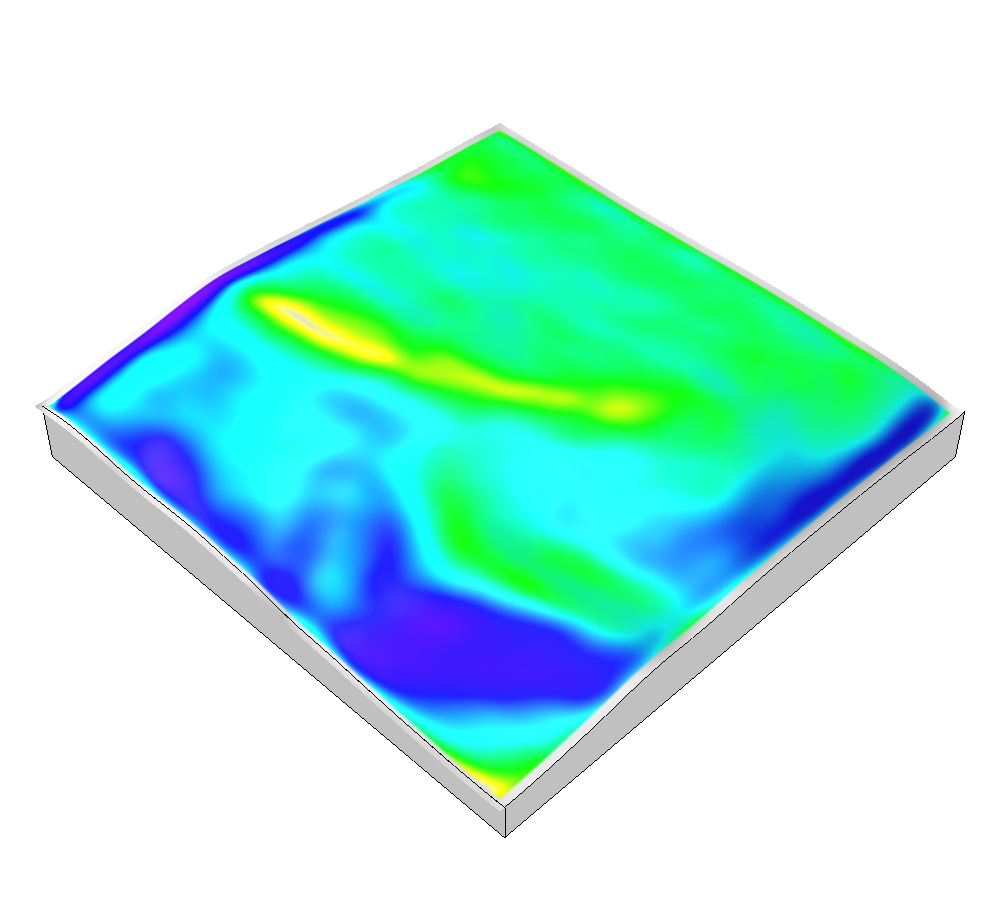
\includegraphics[width=0.22\textwidth]{images/render_3d/mean_slope_4.png} &
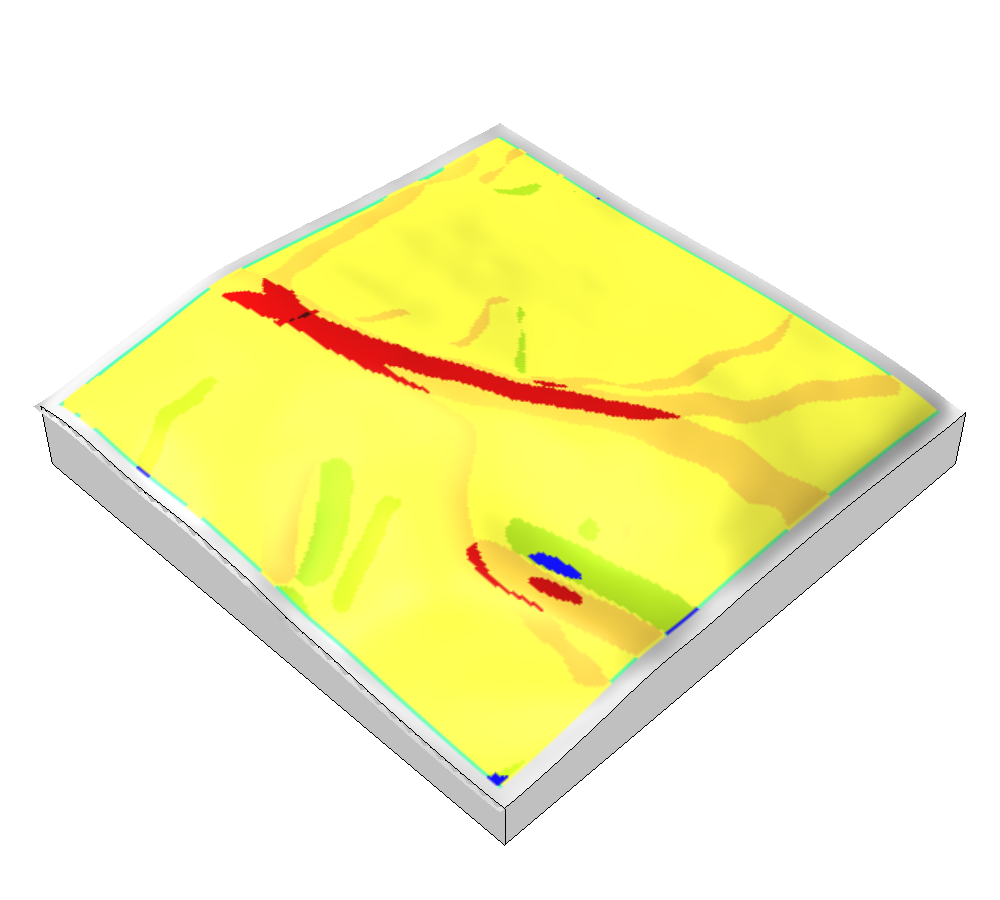
\includegraphics[width=0.22\textwidth]{images/render_3d/mean_forms_4.png}\\
%
&
\multicolumn{1}{c}{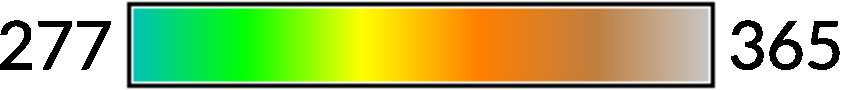
\includegraphics[width=0.22\textwidth]{images/legends/elevation_legend_4.pdf}} &
\multicolumn{1}{c}{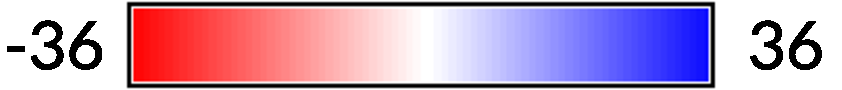
\includegraphics[width=0.22\textwidth]{images/legends/diff_legend.pdf}} &
\multicolumn{1}{c}{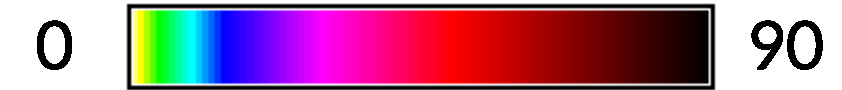
\includegraphics[width=0.22\textwidth]{images/legends/slope_legend.pdf}} &
\multicolumn{1}{c}{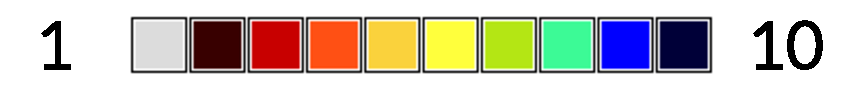
\includegraphics[width=0.22\textwidth]{images/legends/forms_legend.pdf}}\\
%
\bottomrule
\end{tabular}}
\label{table:difference_experiment} 
\end{table}

%%%%%%%%%%%%%%%%%%   WATER FLOW STATS TABLE

\begin{table}
\tbl{Water flow experiment}{
\ra{1.3}
\begin{tabular}{m{0.24\textwidth} m{0.24\textwidth} m{0.24\textwidth} m{0.24\textwidth}}
\toprule
\multicolumn{1}{c}{Reference elevation} & \multicolumn{1}{c}{Mean elevation} & \multicolumn{1}{c}{Stdev.~ of elevations} & \multicolumn{1}{c}{Stdev.~ of differences}\\
\midrule
\includegraphics[width=0.24\textwidth]{images/render_3d/dem_5.png} &
\includegraphics[width=0.24\textwidth]{images/render_3d/mean_dem_5.png} &
\includegraphics[width=0.24\textwidth]{images/render_3d/stdev_dem_5.png} &
\includegraphics[width=0.24\textwidth]{images/render_3d/stdev_regression_difference_series_5.png}\\
%
\multicolumn{1}{c}{\includegraphics[width=0.22\textwidth]{images/legends/elevation_legend_5.pdf}} &
\multicolumn{1}{c}{\includegraphics[width=0.22\textwidth]{images/legends/elevation_legend_5.pdf}} &
\multicolumn{1}{c}{\includegraphics[width=0.22\textwidth]{images/legends/stdev_legend.pdf}} &
\multicolumn{1}{c}{\includegraphics[width=0.22\textwidth]{images/legends/stdev_diff_legend.pdf}}\\
%
\bottomrule
\end{tabular}}
\label{table:water_flow_stats} 
\end{table}

%%%%%%%%%%%%%%%%%% WATER FLOW TABLE

\begin{table}
\tbl{Water flow experiment}{
\ra{1.3}
\begin{tabular}{m{0.1\textwidth} m{0.3\textwidth} m{0.3\textwidth} m{0.3\textwidth}}
\toprule
& \multicolumn{1}{c}{Elevation} & \multicolumn{1}{c}{Water depth} & \multicolumn{1}{c}{Depth difference}\\
\midrule
%
Reference & 
\includegraphics[width=0.3\textwidth]{images/render_3d/dem_5.png} &
\includegraphics[width=0.3\textwidth]{images/render_3d/depth_5.png} &
\includegraphics[width=0.3\textwidth]{images/render_3d/dem_difference_5.png}\\
%
Mean & 
\includegraphics[width=0.3\textwidth]{images/render_3d/mean_dem_5.png} &
\includegraphics[width=0.3\textwidth]{images/render_3d/mean_depth_5.png} &
\includegraphics[width=0.3\textwidth]{images/render_3d/mean_depth_difference_5.png}\\
%
& 
\multicolumn{1}{c}{\includegraphics[width=0.22\textwidth]{images/legends/elevation_legend_5.pdf}} &
\multicolumn{1}{c}{\includegraphics[width=0.22\textwidth]{images/legends/depth_legend.pdf}} &
\multicolumn{1}{c}{\includegraphics[width=0.22\textwidth]{images/legends/depth_diff_legend.pdf}}\\
%
\bottomrule
\end{tabular}}
\label{table:water_flow_experiment} 
\end{table}


% \caption{Water flow experiment: reference elevation, mean elevation, standard deviation of elevations, and standard deviation of linearly regressed differences}

%%%%%%%%%%%%%%%%%%   WATER FLOW TABLE

%\begin{table}
%\tbl{Water flow experiment}{
%\ra{1.3}
%\begin{tabular}{m{0.18\textwidth} m{0.4\textwidth} m{0.4\textwidth}}
%\toprule
%& \multicolumn{1}{c}{Reference} & \multicolumn{1}{c}{Mean}\\
%\midrule
%Elevation & \includegraphics[width=0.4\textwidth]{images/render_3d/dem_5.png} & \includegraphics[width=0.4\textwidth]{images/render_3d/mean_dem_5.png}\\
%Water depth & \includegraphics[width=0.4\textwidth]{images/render_3d/depth_5.png} & \includegraphics[width=0.4\textwidth]{images/render_3d/mean_depth_5.png}\\
%Depth difference & \includegraphics[width=0.4\textwidth]{images/render_3d/dem_difference_5.png} & \includegraphics[width=0.4\textwidth]{images/render_3d/mean_depth_difference_5.png}\\
%\bottomrule
%\end{tabular}}
%\label{table:water_flow_experiment} 
%\end{table}

%%%%%%%%%%%%%%%%%%   WATER FLOW

%\begin{figure*}[h!]
%\begin{center}
%		\includegraphics[width=0.32\textwidth]{images/render_3d/dem_5.png}
%		\includegraphics[width=0.32\textwidth]{images/render_3d/mean_dem_5.png}
%		\includegraphics[width=0.32\textwidth]{images/render_3d/stdev_dem_5.png}
%	\caption{Water flow experiment: reference elevation, mean elevation, and standard deviation of elevations}
%	\label{fig:}
%\end{center}
%\end{figure*}

%\begin{figure*}[h!]
%\begin{center}
%		\includegraphics[width=0.48\textwidth]{images/render_3d/dem_5.png}
%		\includegraphics[width=0.48\textwidth]{images/render_3d/mean_dem_5.png}
%		\includegraphics[width=0.48\textwidth]{images/render_3d/depth_5.png}
%		\includegraphics[width=0.48\textwidth]{images/render_3d/mean_depth_5.png}
%		\includegraphics[width=0.48\textwidth]{images/render_3d/dem_difference_5.png}
%		\includegraphics[width=0.48\textwidth]{images/render_3d/mean_depth_difference_5.png}
%	\caption{Water flow experiment}
%	\label{fig:}
%\end{center}
%\end{figure*}




%\begin{tabular}{*{2}{m{0.48\textwidth}}}
%\hline
%This is some text&\begin{center}\rule{0.4\textwidth}{0.3\textwidth}\end{center}\\

%%%%%%%%%%%%%%%%%%   EXPERIMENT 1-3 WITH LINEAR REGRESSION

%\begin{figure*}[h!]
%\begin{center}
%		%
%		% dem
%		\includegraphics[width=0.24\textwidth]{images/render_3d/dem_1.png}
%		\includegraphics[width=0.24\textwidth]{images/render_3d/mean_dem_regression_1.png}
%		\includegraphics[width=0.24\textwidth]{images/render_3d/mean_dem_regression_2.png}
%		\includegraphics[width=0.24\textwidth]{images/render_3d/mean_dem_regression_3.png}
%		%
%		% difference
%		\includegraphics[width=0.24\textwidth]{images/render_3d/dem_difference_1.png}
%		\includegraphics[width=0.24\textwidth]{images/render_3d/mean_dem_regression_difference_1.png}
%		\includegraphics[width=0.24\textwidth]{images/render_3d/mean_dem_regression_difference_2.png}
%		\includegraphics[width=0.24\textwidth]{images/render_3d/mean_dem_regression_difference_3.png}
%		%
%		% slope
%		\includegraphics[width=0.24\textwidth]{images/render_3d/slope_1.png}
%		\includegraphics[width=0.24\textwidth]{images/render_3d/mean_slope_regression_1.png}
%		\includegraphics[width=0.24\textwidth]{images/render_3d/mean_slope_regression_2.png}
%		\includegraphics[width=0.24\textwidth]{images/render_3d/mean_slope_regression_3.png}
%		%
%		% form
%		\includegraphics[width=0.24\textwidth]{images/render_3d/forms_1.png}
%		\includegraphics[width=0.24\textwidth]{images/render_3d/mean_forms_1.png} % mean_forms_regression_1.png
%		\includegraphics[width=0.24\textwidth]{images/render_3d/mean_forms_2.png} % mean_forms_regression_2.png
%		\includegraphics[width=0.24\textwidth]{images/render_3d/mean_forms_3.png}  % mean_forms_regression_3.png
%		%
%		% depth
%		\includegraphics[width=0.24\textwidth]{images/render_3d/depth_1.png}
%		\includegraphics[width=0.24\textwidth]{images/render_3d/mean_depth_1.png} % mean_depth_regression_1.png
%		\includegraphics[width=0.24\textwidth]{images/render_3d/mean_depth_2.png} % mean_depth_regression_2.png
%		\includegraphics[width=0.24\textwidth]{images/render_3d/mean_depth_3.png} % mean_depth_regression_3.png
%		%
%	\caption{...}
%	\label{fig:}
%\end{center}
%\end{figure*}

%%%%%%%%%%%%%%%%%%  MASTER

%\begin{figure*}[h!]
%\begin{center}
%		%
%		\includegraphics[width=0.18\textwidth]{images/render_3d/dem_1.png}
%		\includegraphics[width=0.18\textwidth]{images/render_3d/dem_2.png}
%		\includegraphics[width=0.18\textwidth]{images/render_3d/dem_3.png}
%		\includegraphics[width=0.18\textwidth]{images/render_3d/dem_4.png}
%		\includegraphics[width=0.18\textwidth]{images/render_3d/dem_5.png}
%		%
%		\includegraphics[width=0.18\textwidth]{images/render_3d/mean_dem_1.png}
%		\includegraphics[width=0.18\textwidth]{images/render_3d/mean_dem_2.png}
%		\includegraphics[width=0.18\textwidth]{images/render_3d/mean_dem_3.png}
%		\includegraphics[width=0.18\textwidth]{images/render_3d/mean_dem_4.png}
%		\includegraphics[width=0.18\textwidth]{images/render_3d/mean_dem_5.png}
%		%
%		\includegraphics[width=0.18\textwidth]{images/render_3d/mean_dem_difference_1.png}
%		\includegraphics[width=0.18\textwidth]{images/render_3d/mean_dem_difference_2.png}
%		\includegraphics[width=0.18\textwidth]{images/render_3d/mean_dem_difference_3.png}
%		\includegraphics[width=0.18\textwidth]{images/render_3d/mean_dem_difference_4.png}
%		\includegraphics[width=0.18\textwidth]{images/render_3d/mean_dem_difference_5.png}
%		%
%		\includegraphics[width=0.18\textwidth]{images/render_3d/mean_slope_1.png}
%		\includegraphics[width=0.18\textwidth]{images/render_3d/mean_slope_2.png}
%		\includegraphics[width=0.18\textwidth]{images/render_3d/mean_slope_3.png}
%		\includegraphics[width=0.18\textwidth]{images/render_3d/mean_slope_4.png}
%		\includegraphics[width=0.18\textwidth]{images/render_3d/mean_slope_5.png}
%		%
%		\includegraphics[width=0.18\textwidth]{images/render_3d/mean_forms_1.png}
%		\includegraphics[width=0.18\textwidth]{images/render_3d/mean_forms_2.png}
%		\includegraphics[width=0.18\textwidth]{images/render_3d/mean_forms_3.png}
%		\includegraphics[width=0.18\textwidth]{images/render_3d/mean_forms_4.png}
%		\includegraphics[width=0.18\textwidth]{images/render_3d/mean_forms_5.png}
%		%
%		\includegraphics[width=0.18\textwidth]{images/render_3d/mean_depth_1.png}
%		\includegraphics[width=0.18\textwidth]{images/render_3d/mean_depth_2.png}
%		\includegraphics[width=0.18\textwidth]{images/render_3d/mean_depth_3.png}
%		\includegraphics[width=0.18\textwidth]{images/render_3d/mean_depth_4.png}
%		\includegraphics[width=0.18\textwidth]{images/render_3d/mean_depth_5.png}
%		%
%		\includegraphics[width=0.18\textwidth]{images/render_3d/mean_depth_difference_1.png}
%		\includegraphics[width=0.18\textwidth]{images/render_3d/mean_depth_difference_2.png}
%		\includegraphics[width=0.18\textwidth]{images/render_3d/mean_depth_difference_3.png}
%		\includegraphics[width=0.18\textwidth]{images/render_3d/mean_depth_difference_4.png}
%		\includegraphics[width=0.18\textwidth]{images/render_3d/mean_depth_difference_5.png}
%		%
%	\caption{...}
%	\label{fig:}
%\end{center}
%\end{figure*}




%%%%%%%%%%%%%%%%%% EXPERIMENT 1 - 3

%\begin{figure*}[h!]
%\begin{center}
%		%
%		% dem
%		\includegraphics[width=0.24\textwidth]{images/render_3d/dem_1.png}
%		\includegraphics[width=0.24\textwidth]{images/render_3d/mean_dem_1.png}
%		\includegraphics[width=0.24\textwidth]{images/render_3d/mean_dem_2.png}
%		\includegraphics[width=0.24\textwidth]{images/render_3d/mean_dem_3.png}
%		%
%		% stdev dem
%		\includegraphics[width=0.24\textwidth]{images/render_3d/dem_difference_1.png}
%		\includegraphics[width=0.24\textwidth]{images/render_3d/stdev_dem_1.png}
%		\includegraphics[width=0.24\textwidth]{images/render_3d/stdev_dem_2.png}
%		\includegraphics[width=0.24\textwidth]{images/render_3d/stdev_dem_3.png}
%		%
%		% difference
%%		\includegraphics[width=0.24\textwidth]{images/render_3d/dem_difference_1.png}
%%		\includegraphics[width=0.24\textwidth]{images/render_3d/mean_dem_difference_1.png}
%%		\includegraphics[width=0.24\textwidth]{images/render_3d/mean_dem_difference_2.png}
%%		\includegraphics[width=0.24\textwidth]{images/render_3d/mean_dem_difference_3.png}
%		%
%		% regression difference
%		\includegraphics[width=0.24\textwidth]{images/render_3d/dem_difference_1.png}
%		\includegraphics[width=0.24\textwidth]{images/render_3d/mean_dem_regression_difference_1.png}
%		\includegraphics[width=0.24\textwidth]{images/render_3d/mean_dem_regression_difference_2.png}
%		\includegraphics[width=0.24\textwidth]{images/render_3d/mean_dem_regression_difference_3.png}
%		%
%		% slope
%		\includegraphics[width=0.24\textwidth]{images/render_3d/slope_1.png}
%		\includegraphics[width=0.24\textwidth]{images/render_3d/mean_slope_1.png}
%		\includegraphics[width=0.24\textwidth]{images/render_3d/mean_slope_2.png}
%		\includegraphics[width=0.24\textwidth]{images/render_3d/mean_slope_3.png}
%		%
%		% form
%		\includegraphics[width=0.24\textwidth]{images/render_3d/forms_1.png}
%		\includegraphics[width=0.24\textwidth]{images/render_3d/mean_forms_1.png}
%		\includegraphics[width=0.24\textwidth]{images/render_3d/mean_forms_2.png}
%		\includegraphics[width=0.24\textwidth]{images/render_3d/mean_forms_3.png}
%		%
%		% depth
%		\includegraphics[width=0.24\textwidth]{images/render_3d/depth_1.png}
%		\includegraphics[width=0.24\textwidth]{images/render_3d/mean_depth_1.png}
%		\includegraphics[width=0.24\textwidth]{images/render_3d/mean_depth_2.png}
%		\includegraphics[width=0.24\textwidth]{images/render_3d/mean_depth_3.png}
%		%
%	\caption{...}
%	\label{fig:coupling_experiment}
%\end{center}
%\end{figure*}


%%%%%%%%%%%%%%%%%%   DIFFERENCE TABLE

%\begin{table}
%\tbl{Difference experiment}{
%\ra{1.3}
%\begin{tabular}{m{0.2\textwidth} m{0.2\textwidth} m{0.2\textwidth} m{0.2\textwidth}}
%\toprule
%\multicolumn{1}{c}{Reference elevation} & \multicolumn{1}{c}{Mean elevation} & \multicolumn{1}{c}{Stdev.~ of elevations}  & \multicolumn{1}{c}{Stdev.~ of differences}\\
%\midrule
%%
%\includegraphics[width=0.24\textwidth]{images/render_3d/dem_4.png} &
%\includegraphics[width=0.24\textwidth]{images/render_3d/mean_dem_4.png} &
%\includegraphics[width=0.24\textwidth]{images/render_3d/stdev_dem_4.png} &
%\includegraphics[width=0.24\textwidth]{images/render_3d/stdev_regression_difference_series_4.png}\\
%%
%\bottomrule
%\end{tabular}}
%\label{table:difference_experiment} 
%\end{table}



%%%%%%%%%%%%%%%%%%   DIFFERENCE

%\begin{figure*}[h!]
%\begin{center}
%		\includegraphics[width=0.32\textwidth]{images/render_3d/dem_4.png}
%		\includegraphics[width=0.32\textwidth]{images/render_3d/mean_dem_4.png}
%		\includegraphics[width=0.32\textwidth]{images/render_3d/stdev_dem_4.png}
%	\caption{Difference experiment: reference elevation, mean elevation, and standard deviation of elevations}
%	\label{fig:}
%\end{center}
%\end{figure*}

%\begin{figure*}[h!]
%\begin{center}
%		\includegraphics[width=0.225\textwidth]{images/render_3d/dem_4.png}
%		\includegraphics[width=0.225\textwidth]{images/render_3d/mean_dem_4.png}
%		\includegraphics[width=0.225\textwidth]{images/render_3d/stdev_dem_4.png}
%		\includegraphics[width=0.225\textwidth]{images/render_3d/stdev_regression_difference_series_4.png}
%	\caption{Difference experiment: reference elevation, mean elevation, standard deviation of elevations, and standard deviation of linearly regressed differences}
%	\label{fig:}
%\end{center}
%\end{figure*}


%%%%%%%%%%%%%%%%%% DIFFERENCE TABLE VERTICAL

%\begin{table}
%\tbl{Difference experiment}{
%\ra{1.3}
%\begin{tabular}{m{0.16\textwidth} m{0.4\textwidth} m{0.4\textwidth}}
%\toprule
%& \multicolumn{1}{c}{Reference} & \multicolumn{1}{c}{Mean}\\
%\midrule
%%
%Elevation & 
%\includegraphics[width=0.4\textwidth]{images/render_3d/dem_4.png} &
%\includegraphics[width=0.4\textwidth]{images/render_3d/mean_dem_4.png}\\
%%
%Elevation difference & 
%\includegraphics[width=0.4\textwidth]{images/render_3d/dem_difference_4.png} &
%\includegraphics[width=0.4\textwidth]{images/render_3d/mean_dem_difference_4.png}\\
%%
%Slope & 
%\includegraphics[width=0.4\textwidth]{images/render_3d/slope_4.png} &
%\includegraphics[width=0.4\textwidth]{images/render_3d/mean_slope_4.png}\\
%%
%Landforms & 
%\includegraphics[width=0.4\textwidth]{images/render_3d/forms_4.png} &
%\includegraphics[width=0.4\textwidth]{images/render_3d/mean_forms_4.png}\\
%%
%\bottomrule
%\end{tabular}}
%\label{table:difference_experiment} 
%\end{table}

%%%%%%%%%%%%%%%%%%   COUPLING TABLE
%
%\begin{table}
%\tbl{Coupling experiment}{
%\ra{1.3}
%\begin{tabular}{m{0.16\textwidth} m{0.2\textwidth} m{0.2\textwidth} m{0.2\textwidth} m{0.2\textwidth}}
%\toprule
%& \multicolumn{1}{c}{Reference} & \multicolumn{1}{c}{Digital} & \multicolumn{1}{c}{Analog}  & \multicolumn{1}{c}{Augmented}\\
%\midrule
%%
%Elevation & 
%\includegraphics[width=0.24\textwidth]{images/render_3d/dem_1.png} &
%\includegraphics[width=0.24\textwidth]{images/render_3d/mean_dem_1.png} &
%\includegraphics[width=0.24\textwidth]{images/render_3d/mean_dem_2.png} &
%\includegraphics[width=0.24\textwidth]{images/render_3d/mean_dem_3.png}\\
%%
%Standard deviation of elevation &
%\includegraphics[width=0.24\textwidth]{images/render_3d/dem_difference_1.png} &
%\includegraphics[width=0.24\textwidth]{images/render_3d/stdev_dem_1.png} &
%\includegraphics[width=0.24\textwidth]{images/render_3d/stdev_dem_2.png} &
%\includegraphics[width=0.24\textwidth]{images/render_3d/stdev_dem_3.png}\\
%%
%Elevation difference &
%\includegraphics[width=0.24\textwidth]{images/render_3d/dem_difference_1.png} &
%\includegraphics[width=0.24\textwidth]{images/render_3d/mean_dem_regression_difference_1.png} &
%\includegraphics[width=0.24\textwidth]{images/render_3d/mean_dem_regression_difference_2.png} &
%\includegraphics[width=0.24\textwidth]{images/render_3d/mean_dem_regression_difference_3.png}\\
%%
%Slope &
%\includegraphics[width=0.24\textwidth]{images/render_3d/slope_1.png} &
%\includegraphics[width=0.24\textwidth]{images/render_3d/mean_slope_1.png} &
%\includegraphics[width=0.24\textwidth]{images/render_3d/mean_slope_2.png} &
%\includegraphics[width=0.24\textwidth]{images/render_3d/mean_slope_3.png}\\
%%
%Landforms &
%\includegraphics[width=0.24\textwidth]{images/render_3d/forms_1.png} &
%\includegraphics[width=0.24\textwidth]{images/render_3d/mean_forms_1.png} &
%\includegraphics[width=0.24\textwidth]{images/render_3d/mean_forms_2.png} &
%\includegraphics[width=0.24\textwidth]{images/render_3d/mean_forms_3.png}\\
%%
%Water flow &
%\includegraphics[width=0.24\textwidth]{images/render_3d/depth_1.png} &
%\includegraphics[width=0.24\textwidth]{images/render_3d/mean_depth_1.png} &
%\includegraphics[width=0.24\textwidth]{images/render_3d/mean_depth_2.png} &
%\includegraphics[width=0.24\textwidth]{images/render_3d/mean_depth_3.png}\\
%%
%\bottomrule
%\end{tabular}}
%\label{table:coupling_experiment} 
%\end{table}

% nota bene: stdev_dem and stdev_difference_series are almost the same!

\end{document}



